\documentclass[]{article}
\usepackage{lmodern}
\usepackage{amssymb,amsmath}
\usepackage{ifxetex,ifluatex}
\usepackage{fixltx2e} % provides \textsubscript
\ifnum 0\ifxetex 1\fi\ifluatex 1\fi=0 % if pdftex
  \usepackage[T1]{fontenc}
  \usepackage[utf8]{inputenc}
\else % if luatex or xelatex
  \ifxetex
    \usepackage{mathspec}
  \else
    \usepackage{fontspec}
  \fi
  \defaultfontfeatures{Ligatures=TeX,Scale=MatchLowercase}
\fi
% use upquote if available, for straight quotes in verbatim environments
\IfFileExists{upquote.sty}{\usepackage{upquote}}{}
% use microtype if available
\IfFileExists{microtype.sty}{%
\usepackage{microtype}
\UseMicrotypeSet[protrusion]{basicmath} % disable protrusion for tt fonts
}{}
\usepackage[margin=1in]{geometry}
\usepackage{hyperref}
\hypersetup{unicode=true,
            pdftitle={Analysis on Ethereum blockchain},
            pdfborder={0 0 0},
            breaklinks=true}
\urlstyle{same}  % don't use monospace font for urls
\usepackage{color}
\usepackage{fancyvrb}
\newcommand{\VerbBar}{|}
\newcommand{\VERB}{\Verb[commandchars=\\\{\}]}
\DefineVerbatimEnvironment{Highlighting}{Verbatim}{commandchars=\\\{\}}
% Add ',fontsize=\small' for more characters per line
\usepackage{framed}
\definecolor{shadecolor}{RGB}{248,248,248}
\newenvironment{Shaded}{\begin{snugshade}}{\end{snugshade}}
\newcommand{\KeywordTok}[1]{\textcolor[rgb]{0.13,0.29,0.53}{\textbf{#1}}}
\newcommand{\DataTypeTok}[1]{\textcolor[rgb]{0.13,0.29,0.53}{#1}}
\newcommand{\DecValTok}[1]{\textcolor[rgb]{0.00,0.00,0.81}{#1}}
\newcommand{\BaseNTok}[1]{\textcolor[rgb]{0.00,0.00,0.81}{#1}}
\newcommand{\FloatTok}[1]{\textcolor[rgb]{0.00,0.00,0.81}{#1}}
\newcommand{\ConstantTok}[1]{\textcolor[rgb]{0.00,0.00,0.00}{#1}}
\newcommand{\CharTok}[1]{\textcolor[rgb]{0.31,0.60,0.02}{#1}}
\newcommand{\SpecialCharTok}[1]{\textcolor[rgb]{0.00,0.00,0.00}{#1}}
\newcommand{\StringTok}[1]{\textcolor[rgb]{0.31,0.60,0.02}{#1}}
\newcommand{\VerbatimStringTok}[1]{\textcolor[rgb]{0.31,0.60,0.02}{#1}}
\newcommand{\SpecialStringTok}[1]{\textcolor[rgb]{0.31,0.60,0.02}{#1}}
\newcommand{\ImportTok}[1]{#1}
\newcommand{\CommentTok}[1]{\textcolor[rgb]{0.56,0.35,0.01}{\textit{#1}}}
\newcommand{\DocumentationTok}[1]{\textcolor[rgb]{0.56,0.35,0.01}{\textbf{\textit{#1}}}}
\newcommand{\AnnotationTok}[1]{\textcolor[rgb]{0.56,0.35,0.01}{\textbf{\textit{#1}}}}
\newcommand{\CommentVarTok}[1]{\textcolor[rgb]{0.56,0.35,0.01}{\textbf{\textit{#1}}}}
\newcommand{\OtherTok}[1]{\textcolor[rgb]{0.56,0.35,0.01}{#1}}
\newcommand{\FunctionTok}[1]{\textcolor[rgb]{0.00,0.00,0.00}{#1}}
\newcommand{\VariableTok}[1]{\textcolor[rgb]{0.00,0.00,0.00}{#1}}
\newcommand{\ControlFlowTok}[1]{\textcolor[rgb]{0.13,0.29,0.53}{\textbf{#1}}}
\newcommand{\OperatorTok}[1]{\textcolor[rgb]{0.81,0.36,0.00}{\textbf{#1}}}
\newcommand{\BuiltInTok}[1]{#1}
\newcommand{\ExtensionTok}[1]{#1}
\newcommand{\PreprocessorTok}[1]{\textcolor[rgb]{0.56,0.35,0.01}{\textit{#1}}}
\newcommand{\AttributeTok}[1]{\textcolor[rgb]{0.77,0.63,0.00}{#1}}
\newcommand{\RegionMarkerTok}[1]{#1}
\newcommand{\InformationTok}[1]{\textcolor[rgb]{0.56,0.35,0.01}{\textbf{\textit{#1}}}}
\newcommand{\WarningTok}[1]{\textcolor[rgb]{0.56,0.35,0.01}{\textbf{\textit{#1}}}}
\newcommand{\AlertTok}[1]{\textcolor[rgb]{0.94,0.16,0.16}{#1}}
\newcommand{\ErrorTok}[1]{\textcolor[rgb]{0.64,0.00,0.00}{\textbf{#1}}}
\newcommand{\NormalTok}[1]{#1}
\usepackage{graphicx,grffile}
\makeatletter
\def\maxwidth{\ifdim\Gin@nat@width>\linewidth\linewidth\else\Gin@nat@width\fi}
\def\maxheight{\ifdim\Gin@nat@height>\textheight\textheight\else\Gin@nat@height\fi}
\makeatother
% Scale images if necessary, so that they will not overflow the page
% margins by default, and it is still possible to overwrite the defaults
% using explicit options in \includegraphics[width, height, ...]{}
\setkeys{Gin}{width=\maxwidth,height=\maxheight,keepaspectratio}
\IfFileExists{parskip.sty}{%
\usepackage{parskip}
}{% else
\setlength{\parindent}{0pt}
\setlength{\parskip}{6pt plus 2pt minus 1pt}
}
\setlength{\emergencystretch}{3em}  % prevent overfull lines
\providecommand{\tightlist}{%
  \setlength{\itemsep}{0pt}\setlength{\parskip}{0pt}}
\setcounter{secnumdepth}{0}
% Redefines (sub)paragraphs to behave more like sections
\ifx\paragraph\undefined\else
\let\oldparagraph\paragraph
\renewcommand{\paragraph}[1]{\oldparagraph{#1}\mbox{}}
\fi
\ifx\subparagraph\undefined\else
\let\oldsubparagraph\subparagraph
\renewcommand{\subparagraph}[1]{\oldsubparagraph{#1}\mbox{}}
\fi

%%% Use protect on footnotes to avoid problems with footnotes in titles
\let\rmarkdownfootnote\footnote%
\def\footnote{\protect\rmarkdownfootnote}

%%% Change title format to be more compact
\usepackage{titling}

% Create subtitle command for use in maketitle
\providecommand{\subtitle}[1]{
  \posttitle{
    \begin{center}\large#1\end{center}
    }
}

\setlength{\droptitle}{-2em}

  \title{Analysis on Ethereum blockchain}
    \pretitle{\vspace{\droptitle}\centering\huge}
  \posttitle{\par}
    \author{}
    \preauthor{}\postauthor{}
    \date{}
    \predate{}\postdate{}
  

\begin{document}
\maketitle

\subsubsection{We have chosen the three tokens as per the criteria
specified in the problem statement. The modulo of sum of team member's
UTD ID by 20 is 3. The top 3rd, 4th and 5th biggest tokens are
networkomisegoTX, networkyocoinTX, and
networkgolemTX}\label{we-have-chosen-the-three-tokens-as-per-the-criteria-specified-in-the-problem-statement.-the-modulo-of-sum-of-team-members-utd-id-by-20-is-3.-the-top-3rd-4th-and-5th-biggest-tokens-are-networkomisegotx-networkyocointx-and-networkgolemtx}

\subsection{Loading libraries}\label{loading-libraries}

\begin{Shaded}
\begin{Highlighting}[]
\KeywordTok{library}\NormalTok{(dplyr)}
\end{Highlighting}
\end{Shaded}

\begin{verbatim}
## 
## Attaching package: 'dplyr'
\end{verbatim}

\begin{verbatim}
## The following objects are masked from 'package:stats':
## 
##     filter, lag
\end{verbatim}

\begin{verbatim}
## The following objects are masked from 'package:base':
## 
##     intersect, setdiff, setequal, union
\end{verbatim}

\begin{Shaded}
\begin{Highlighting}[]
\KeywordTok{library}\NormalTok{(ggplot2)}
\KeywordTok{library}\NormalTok{(fitdistrplus)}
\end{Highlighting}
\end{Shaded}

\begin{verbatim}
## Loading required package: MASS
\end{verbatim}

\begin{verbatim}
## 
## Attaching package: 'MASS'
\end{verbatim}

\begin{verbatim}
## The following object is masked from 'package:dplyr':
## 
##     select
\end{verbatim}

\begin{verbatim}
## Loading required package: survival
\end{verbatim}

\begin{verbatim}
## Loading required package: npsurv
\end{verbatim}

\begin{verbatim}
## Loading required package: lsei
\end{verbatim}

\section{Question 1}\label{question-1}

\subsection{\texorpdfstring{Analysis on token
`networkgolemTX'}{Analysis on token networkgolemTX}}\label{analysis-on-token-networkgolemtx}

\paragraph{Loading token graph edge file into a
dataframe}\label{loading-token-graph-edge-file-into-a-dataframe}

\begin{Shaded}
\begin{Highlighting}[]
\NormalTok{networkgolemTX <-}\StringTok{ }\KeywordTok{read.csv}\NormalTok{(}\StringTok{'data/networkgolemTX.txt'}\NormalTok{, }\DataTypeTok{sep=}\StringTok{" "}\NormalTok{, }\DataTypeTok{header =} \OtherTok{FALSE}\NormalTok{)}
\KeywordTok{names}\NormalTok{(networkgolemTX) <-}\StringTok{ }\KeywordTok{c}\NormalTok{(}\StringTok{"fromAddress"}\NormalTok{, }\StringTok{"toAddress"}\NormalTok{, }\StringTok{"unixTime"}\NormalTok{, }\StringTok{"tokenAmount"}\NormalTok{)}
\KeywordTok{head}\NormalTok{(networkgolemTX)}
\end{Highlighting}
\end{Shaded}

\begin{verbatim}
##   fromAddress toAddress   unixTime  tokenAmount
## 1     2335455    361874 1524611390 8.023884e+18
## 2     4067684   4067685 1524611418 5.000000e+22
## 3       75994   4067686 1524611727 1.114323e+23
## 4      297031   4067687 1524611781 4.661232e+19
## 5       75994   4067688 1524611836 9.063376e+21
## 6     4067689   2335455 1524611836 2.087045e+20
\end{verbatim}

\paragraph{Checking the data type for each
column}\label{checking-the-data-type-for-each-column}

\begin{Shaded}
\begin{Highlighting}[]
\KeywordTok{str}\NormalTok{(networkgolemTX)}
\end{Highlighting}
\end{Shaded}

\begin{verbatim}
## 'data.frame':    684338 obs. of  4 variables:
##  $ fromAddress: int  2335455 4067684 75994 297031 75994 4067689 4067690 40002 75994 2335455 ...
##  $ toAddress  : int  361874 4067685 4067686 4067687 4067688 2335455 2335455 1810 118 3135852 ...
##  $ unixTime   : int  1524611390 1524611418 1524611727 1524611781 1524611836 1524611836 1524611836 1524611948 1524611984 1524612057 ...
##  $ tokenAmount: num  8.02e+18 5.00e+22 1.11e+23 4.66e+19 9.06e+21 ...
\end{verbatim}

\paragraph{All columns have correct data types. We'll now check if there
are any transactions with same
addresses}\label{all-columns-have-correct-data-types.-well-now-check-if-there-are-any-transactions-with-same-addresses}

\begin{Shaded}
\begin{Highlighting}[]
\NormalTok{sameTx <-}\StringTok{ }\NormalTok{networkgolemTX[networkgolemTX}\OperatorTok{$}\NormalTok{fromAddress }\OperatorTok{==}\StringTok{ }\NormalTok{networkgolemTX}\OperatorTok{$}\NormalTok{toAddress, ] }
\CommentTok{#head(sameTx)}
\KeywordTok{nrow}\NormalTok{(sameTx)}
\end{Highlighting}
\end{Shaded}

\begin{verbatim}
## [1] 635
\end{verbatim}

\paragraph{It can be observed that there were 635 transactions that
occured where sender and recipient have the same
address.}\label{it-can-be-observed-that-there-were-635-transactions-that-occured-where-sender-and-recipient-have-the-same-address.}

\begin{Shaded}
\begin{Highlighting}[]
\KeywordTok{nrow}\NormalTok{(}\KeywordTok{unique}\NormalTok{(sameTx[}\StringTok{"fromAddress"}\NormalTok{]))}
\end{Highlighting}
\end{Shaded}

\begin{verbatim}
## [1] 427
\end{verbatim}

\paragraph{We observe that there are 427 unique addresses which have
self transactions.These are malicious user transactions and we'll remove
them from our
analysis.}\label{we-observe-that-there-are-427-unique-addresses-which-have-self-transactions.these-are-malicious-user-transactions-and-well-remove-them-from-our-analysis.}

\begin{Shaded}
\begin{Highlighting}[]
\NormalTok{cleanedGolemTX <-}\StringTok{ }\NormalTok{networkgolemTX[networkgolemTX}\OperatorTok{$}\NormalTok{fromAddress }\OperatorTok{!=}\StringTok{ }\NormalTok{networkgolemTX}\OperatorTok{$}\NormalTok{toAddress, ] }
\end{Highlighting}
\end{Shaded}

\paragraph{\texorpdfstring{Checking if any of the token amount exceeds
the total supply of the coin, which is limited to (1 x 10\^{}9)
(\url{https://coinmarketcap.com/currencies/golem-network-tokens/})}{Checking if any of the token amount exceeds the total supply of the coin, which is limited to (1 x 10\^{}9) (https://coinmarketcap.com/currencies/golem-network-tokens/)}}\label{checking-if-any-of-the-token-amount-exceeds-the-total-supply-of-the-coin-which-is-limited-to-1-x-109-httpscoinmarketcap.comcurrenciesgolem-network-tokens}

\paragraph{Each coin can have upto a maximum of 10\^{}18 subunits.
Therefore, the token amount that can exist in the data should be less
than total supply * 10\^{}18. Anything beyond this amount will be
considered as outliers and removed from
analysis.}\label{each-coin-can-have-upto-a-maximum-of-1018-subunits.-therefore-the-token-amount-that-can-exist-in-the-data-should-be-less-than-total-supply-1018.-anything-beyond-this-amount-will-be-considered-as-outliers-and-removed-from-analysis.}

\begin{Shaded}
\begin{Highlighting}[]
\NormalTok{subUnits <-}\StringTok{ }\DecValTok{10}\OperatorTok{^}\DecValTok{18}
\NormalTok{totalSupply <-}\StringTok{ }\DecValTok{1} \OperatorTok{*}\StringTok{ }\DecValTok{10}\OperatorTok{^}\DecValTok{9}
\NormalTok{outliersDf <-}\StringTok{ }\NormalTok{cleanedGolemTX[cleanedGolemTX}\OperatorTok{$}\NormalTok{tokenAmount }\OperatorTok{>}\StringTok{ }\NormalTok{totalSupply }\OperatorTok{*}\StringTok{ }\NormalTok{subUnits,]}
\KeywordTok{nrow}\NormalTok{(outliersDf)}
\end{Highlighting}
\end{Shaded}

\begin{verbatim}
## [1] 25
\end{verbatim}

\paragraph{It can be observed that for 25 transactions, the token amount
is larger than the expected total supply of the coins. This anomaly can
be attributed to the BatchOverflow Exploit which resulted in generating
astronomical values. We'll remove such transaction from our
analysis.}\label{it-can-be-observed-that-for-25-transactions-the-token-amount-is-larger-than-the-expected-total-supply-of-the-coins.-this-anomaly-can-be-attributed-to-the-batchoverflow-exploit-which-resulted-in-generating-astronomical-values.-well-remove-such-transaction-from-our-analysis.}

\paragraph{\texorpdfstring{After removing the invalid transactions,
we'll generate the `buy' distribution. This will contain the frequency
of number of buys performed by
users}{After removing the invalid transactions, we'll generate the buy distribution. This will contain the frequency of number of buys performed by users}}\label{after-removing-the-invalid-transactions-well-generate-the-buy-distribution.-this-will-contain-the-frequency-of-number-of-buys-performed-by-users}

\begin{Shaded}
\begin{Highlighting}[]
\NormalTok{filteredGolemTX <-}\StringTok{ }\NormalTok{cleanedGolemTX[cleanedGolemTX}\OperatorTok{$}\NormalTok{tokenAmount }\OperatorTok{<=}\StringTok{ }\NormalTok{totalSupply }\OperatorTok{*}\StringTok{ }\NormalTok{subUnits,]}
\CommentTok{#buys.distribution <- filteredGolemTX %>% group_by(toNode) %>% summarise(n = n()) %>% ungroup}
\NormalTok{pair.users.buys <-}\StringTok{ }\NormalTok{filteredGolemTX }\OperatorTok\StringTok{ }\KeywordTok{group_by}\NormalTok{(toAddress) }\OperatorTok\StringTok{ }\KeywordTok{summarise}\NormalTok{(}\DataTypeTok{n =} \KeywordTok{n}\NormalTok{(), }\DataTypeTok{sumAmount=}\KeywordTok{sum}\NormalTok{(tokenAmount)) }\OperatorTok\StringTok{ }\NormalTok{ungroup}
\KeywordTok{head}\NormalTok{(pair.users.buys)}
\end{Highlighting}
\end{Shaded}

\begin{verbatim}
## # A tibble: 6 x 3
##   toAddress     n sumAmount
##       <int> <int>     <dbl>
## 1         5  3709   5.15e25
## 2         6    33   6.74e24
## 3         7   622   2.54e25
## 4         8   345   2.78e25
## 5        13    22   2.50e25
## 6        17    11   5.84e21
\end{verbatim}

\subsubsection{\texorpdfstring{Plotting density distribution for `Buy'
transactions. We'll check if we are able to identify frequency of number
of buys between 2
users}{Plotting density distribution for Buy transactions. We'll check if we are able to identify frequency of number of buys between 2 users}}\label{plotting-density-distribution-for-buy-transactions.-well-check-if-we-are-able-to-identify-frequency-of-number-of-buys-between-2-users}

\begin{Shaded}
\begin{Highlighting}[]
\KeywordTok{ggplot}\NormalTok{(}\DataTypeTok{data=}\NormalTok{pair.users.buys, }\KeywordTok{aes}\NormalTok{(pair.users.buys}\OperatorTok{$}\NormalTok{n)) }\OperatorTok{+}\StringTok{ }
\StringTok{  }\KeywordTok{geom_density}\NormalTok{(}\DataTypeTok{fill=}\StringTok{'yellow'}\NormalTok{, }\DataTypeTok{color=}\StringTok{'yellow'}\NormalTok{) }\OperatorTok{+}\StringTok{ }
\StringTok{  }\KeywordTok{scale_x_continuous}\NormalTok{(}\DataTypeTok{breaks=}\KeywordTok{seq}\NormalTok{(}\DecValTok{0}\NormalTok{,}\DecValTok{15}\NormalTok{,}\DecValTok{1}\NormalTok{), }\DataTypeTok{limits=}\KeywordTok{c}\NormalTok{(}\DecValTok{0}\NormalTok{,}\DecValTok{15}\NormalTok{)) }\OperatorTok{+}\StringTok{ }
\StringTok{  }\KeywordTok{xlab}\NormalTok{(}\StringTok{"No. of buys (Pair-wise)"}\NormalTok{) }\OperatorTok{+}
\StringTok{  }\KeywordTok{ylab}\NormalTok{(}\StringTok{"Density"}\NormalTok{) }\OperatorTok{+}\StringTok{ }
\StringTok{  }\KeywordTok{ggtitle}\NormalTok{(}\StringTok{"Buy Distribution"}\NormalTok{) }\OperatorTok{+}
\StringTok{  }\KeywordTok{theme}\NormalTok{(}\DataTypeTok{text =} \KeywordTok{element_text}\NormalTok{(}\DataTypeTok{color =} \StringTok{"#444444"}\NormalTok{)}
\NormalTok{        ,}\DataTypeTok{panel.background =} \KeywordTok{element_rect}\NormalTok{(}\DataTypeTok{fill =} \StringTok{'#444B5A'}\NormalTok{)}
\NormalTok{        ,}\DataTypeTok{panel.grid.minor =} \KeywordTok{element_line}\NormalTok{(}\DataTypeTok{color =} \StringTok{'#4d5566'}\NormalTok{)}
\NormalTok{        ,}\DataTypeTok{panel.grid.major =} \KeywordTok{element_line}\NormalTok{(}\DataTypeTok{color =} \StringTok{'#586174'}\NormalTok{)}
\NormalTok{        ,}\DataTypeTok{plot.title =} \KeywordTok{element_text}\NormalTok{(}\DataTypeTok{size =} \DecValTok{24}\NormalTok{)}
\NormalTok{        ,}\DataTypeTok{axis.title =} \KeywordTok{element_text}\NormalTok{(}\DataTypeTok{size =} \DecValTok{18}\NormalTok{, }\DataTypeTok{color =} \StringTok{'#555555'}\NormalTok{)}
\NormalTok{        ,}\DataTypeTok{axis.title.y =} \KeywordTok{element_text}\NormalTok{(}\DataTypeTok{vjust =}\NormalTok{ .}\DecValTok{5}\NormalTok{, }\DataTypeTok{angle =} \DecValTok{0}\NormalTok{)}
\NormalTok{        ,}\DataTypeTok{axis.title.x =} \KeywordTok{element_text}\NormalTok{(}\DataTypeTok{hjust =}\NormalTok{ .}\DecValTok{5}\NormalTok{)}
\NormalTok{  ) }
\end{Highlighting}
\end{Shaded}

\begin{verbatim}
## Warning: Removed 1747 rows containing non-finite values (stat_density).
\end{verbatim}

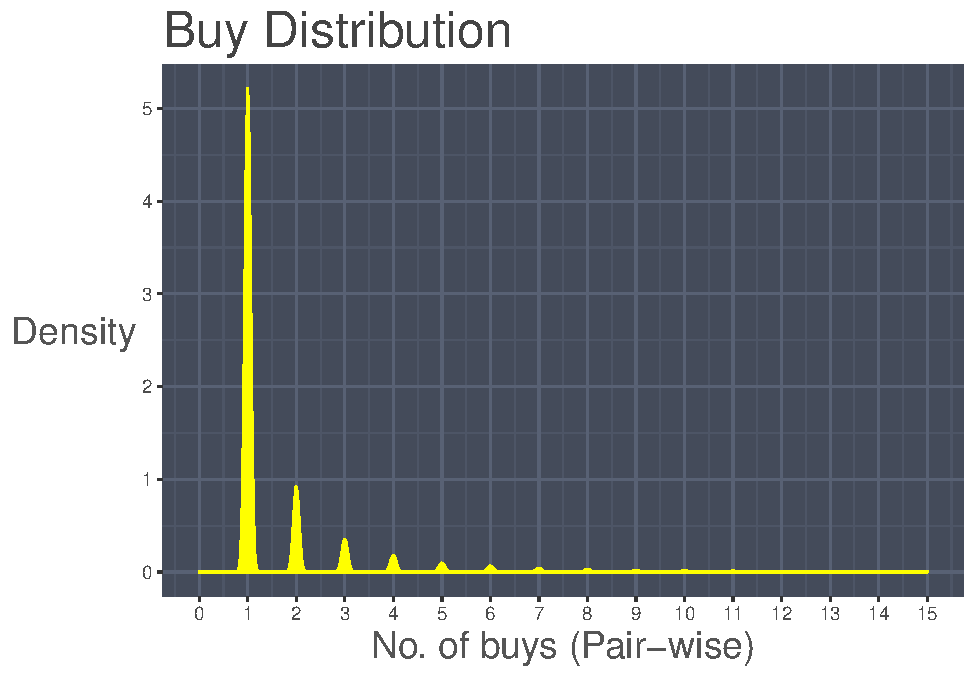
\includegraphics{analysis_files/figure-latex/unnamed-chunk-9-1.pdf}

\subsubsection{\texorpdfstring{Similarly, we'll generate the `sell'
distribution. This will contain the frequency of number of sells
performed by
users}{Similarly, we'll generate the sell distribution. This will contain the frequency of number of sells performed by users}}\label{similarly-well-generate-the-sell-distribution.-this-will-contain-the-frequency-of-number-of-sells-performed-by-users}

\begin{Shaded}
\begin{Highlighting}[]
\NormalTok{pair.users.sells <-}\StringTok{ }\NormalTok{filteredGolemTX }\OperatorTok\StringTok{ }\KeywordTok{group_by}\NormalTok{(fromAddress) }\OperatorTok\StringTok{ }\KeywordTok{summarise}\NormalTok{(}\DataTypeTok{n =} \KeywordTok{n}\NormalTok{(), }\DataTypeTok{sumAmount=}\KeywordTok{sum}\NormalTok{(tokenAmount))}
\KeywordTok{head}\NormalTok{(pair.users.sells)}
\end{Highlighting}
\end{Shaded}

\begin{verbatim}
## # A tibble: 6 x 3
##   fromAddress     n sumAmount
##         <int> <int>     <dbl>
## 1           5   808   5.15e25
## 2           6   620   6.71e24
## 3           7   195   2.54e25
## 4           8  1074   2.25e25
## 5          13  3528   5.26e25
## 6          17 67975   4.25e26
\end{verbatim}

\subsubsection{\texorpdfstring{Plotting density distribution for `Sell'
transactions}{Plotting density distribution for Sell transactions}}\label{plotting-density-distribution-for-sell-transactions}

\begin{Shaded}
\begin{Highlighting}[]
\KeywordTok{ggplot}\NormalTok{(}\DataTypeTok{data=}\NormalTok{pair.users.sells, }\KeywordTok{aes}\NormalTok{(pair.users.sells}\OperatorTok{$}\NormalTok{n)) }\OperatorTok{+}\StringTok{ }
\StringTok{  }\KeywordTok{geom_density}\NormalTok{(}\DataTypeTok{fill=}\StringTok{'cyan'}\NormalTok{, }\DataTypeTok{color=}\StringTok{'cyan'}\NormalTok{) }\OperatorTok{+}\StringTok{ }
\StringTok{  }\KeywordTok{scale_x_continuous}\NormalTok{(}\DataTypeTok{breaks=}\KeywordTok{seq}\NormalTok{(}\DecValTok{0}\NormalTok{,}\DecValTok{15}\NormalTok{,}\DecValTok{1}\NormalTok{), }\DataTypeTok{limits=}\KeywordTok{c}\NormalTok{(}\DecValTok{0}\NormalTok{,}\DecValTok{15}\NormalTok{)) }\OperatorTok{+}\StringTok{ }
\StringTok{  }\KeywordTok{xlab}\NormalTok{(}\StringTok{"No. of sells (Pair-wise)"}\NormalTok{) }\OperatorTok{+}
\StringTok{  }\KeywordTok{ylab}\NormalTok{(}\StringTok{"Density"}\NormalTok{) }\OperatorTok{+}\StringTok{ }
\StringTok{  }\KeywordTok{ggtitle}\NormalTok{(}\StringTok{"Sell Distribution"}\NormalTok{) }\OperatorTok{+}\StringTok{ }
\StringTok{  }\KeywordTok{theme}\NormalTok{(}\DataTypeTok{text =} \KeywordTok{element_text}\NormalTok{(}\DataTypeTok{color =} \StringTok{"#444444"}\NormalTok{)}
\NormalTok{        ,}\DataTypeTok{panel.background =} \KeywordTok{element_rect}\NormalTok{(}\DataTypeTok{fill =} \StringTok{'#444B5A'}\NormalTok{)}
\NormalTok{        ,}\DataTypeTok{panel.grid.minor =} \KeywordTok{element_line}\NormalTok{(}\DataTypeTok{color =} \StringTok{'#4d5566'}\NormalTok{)}
\NormalTok{        ,}\DataTypeTok{panel.grid.major =} \KeywordTok{element_line}\NormalTok{(}\DataTypeTok{color =} \StringTok{'#586174'}\NormalTok{)}
\NormalTok{        ,}\DataTypeTok{plot.title =} \KeywordTok{element_text}\NormalTok{(}\DataTypeTok{size =} \DecValTok{24}\NormalTok{)}
\NormalTok{        ,}\DataTypeTok{axis.title =} \KeywordTok{element_text}\NormalTok{(}\DataTypeTok{size =} \DecValTok{18}\NormalTok{, }\DataTypeTok{color =} \StringTok{'#555555'}\NormalTok{)}
\NormalTok{        ,}\DataTypeTok{axis.title.y =} \KeywordTok{element_text}\NormalTok{(}\DataTypeTok{vjust =}\NormalTok{ .}\DecValTok{5}\NormalTok{, }\DataTypeTok{angle =} \DecValTok{0}\NormalTok{)}
\NormalTok{        ,}\DataTypeTok{axis.title.x =} \KeywordTok{element_text}\NormalTok{(}\DataTypeTok{hjust =}\NormalTok{ .}\DecValTok{5}\NormalTok{)}
\NormalTok{  ) }
\end{Highlighting}
\end{Shaded}

\begin{verbatim}
## Warning: Removed 1229 rows containing non-finite values (stat_density).
\end{verbatim}

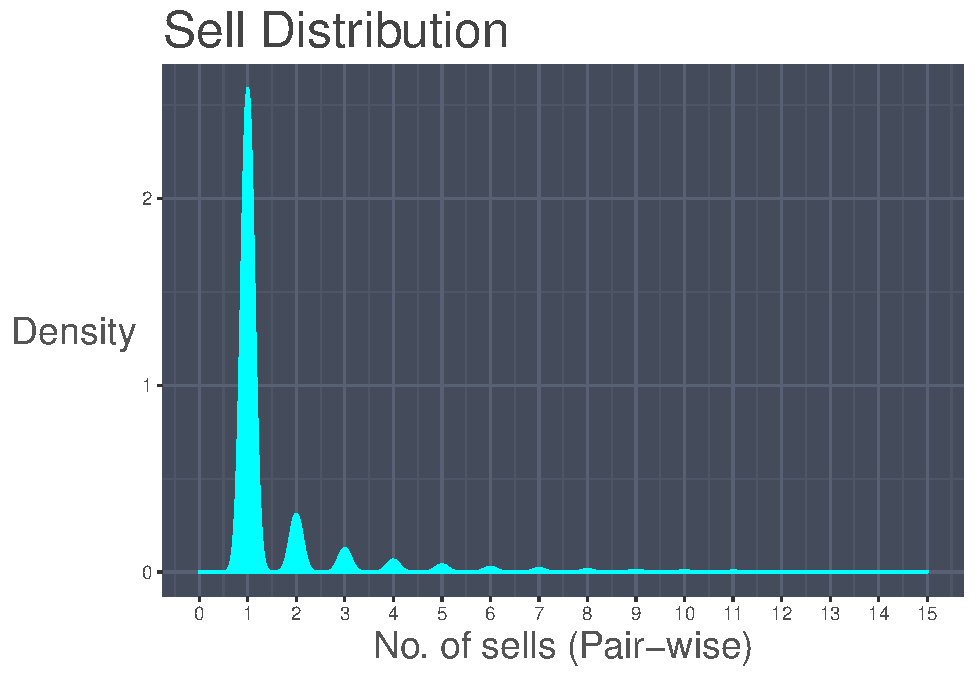
\includegraphics{analysis_files/figure-latex/unnamed-chunk-11-1.pdf}

\subsubsection{Now that we have seen density distributions for both
types of transactions, we'll individually fit the data in different
distribution
models}\label{now-that-we-have-seen-density-distributions-for-both-types-of-transactions-well-individually-fit-the-data-in-different-distribution-models}

\begin{Shaded}
\begin{Highlighting}[]
\NormalTok{fit.buy.norm <-}\StringTok{ }\KeywordTok{fitdist}\NormalTok{(pair.users.buys}\OperatorTok{$}\NormalTok{n, }\StringTok{"norm"}\NormalTok{)}
\NormalTok{fit.buy.weibull  <-}\StringTok{ }\KeywordTok{fitdist}\NormalTok{(pair.users.buys}\OperatorTok{$}\NormalTok{n, }\StringTok{"weibull"}\NormalTok{)}
\NormalTok{fit.buy.gamma  <-}\StringTok{ }\KeywordTok{fitdist}\NormalTok{(pair.users.buys}\OperatorTok{$}\NormalTok{n, }\StringTok{"gamma"}\NormalTok{)}
\NormalTok{fit.buy.lnorm <-}\StringTok{ }\KeywordTok{fitdist}\NormalTok{(pair.users.buys}\OperatorTok{$}\NormalTok{n, }\StringTok{"lnorm"}\NormalTok{)}
\NormalTok{fit.buy.exp <-}\StringTok{ }\KeywordTok{fitdist}\NormalTok{(pair.users.buys}\OperatorTok{$}\NormalTok{n, }\StringTok{"exp"}\NormalTok{)}
\NormalTok{fit.buy.logis <-}\StringTok{ }\KeywordTok{fitdist}\NormalTok{(pair.users.buys}\OperatorTok{$}\NormalTok{n, }\StringTok{"logis"}\NormalTok{)}
\end{Highlighting}
\end{Shaded}

\paragraph{\texorpdfstring{Plotting all distributions and check which
one satisfies our `Buy'
distribution}{Plotting all distributions and check which one satisfies our Buy distribution}}\label{plotting-all-distributions-and-check-which-one-satisfies-our-buy-distribution}

\begin{Shaded}
\begin{Highlighting}[]
\CommentTok{#par(mfrow=c(2,2))}
\NormalTok{plot.legend <-}\StringTok{ }\KeywordTok{c}\NormalTok{(}\StringTok{"Normal"}\NormalTok{, }\StringTok{"Weibull"}\NormalTok{, }\StringTok{"lognormal"}\NormalTok{, }\StringTok{"gamma"}\NormalTok{, }\StringTok{"exponential"}\NormalTok{, }\StringTok{"logistic"}\NormalTok{)}
\KeywordTok{denscomp}\NormalTok{(}\KeywordTok{list}\NormalTok{(fit.buy.norm,fit.buy.weibull , fit.buy.lnorm, fit.buy.gamma, fit.buy.exp,fit.buy.logis), }\DataTypeTok{legendtext =}\NormalTok{ plot.legend, }\DataTypeTok{xlim=}\KeywordTok{c}\NormalTok{(}\DecValTok{0}\NormalTok{,}\DecValTok{15}\NormalTok{), }\DataTypeTok{ylim=}\KeywordTok{c}\NormalTok{(}\DecValTok{0}\NormalTok{,}\DecValTok{1}\NormalTok{))}
\end{Highlighting}
\end{Shaded}

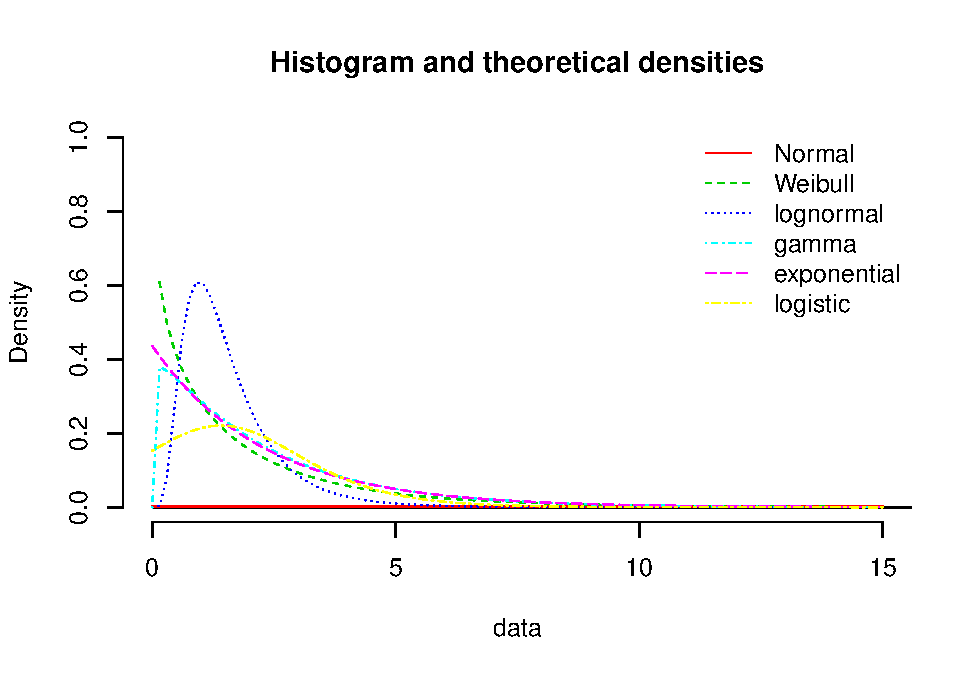
\includegraphics{analysis_files/figure-latex/unnamed-chunk-13-1.pdf}

\begin{Shaded}
\begin{Highlighting}[]
\KeywordTok{gofstat}\NormalTok{(}\KeywordTok{list}\NormalTok{(fit.buy.norm,fit.buy.weibull , fit.buy.lnorm, fit.buy.gamma, fit.buy.exp,fit.buy.logis),}\DataTypeTok{fitnames =} \KeywordTok{c}\NormalTok{(}\StringTok{"Normal"}\NormalTok{, }\StringTok{"Weibull"}\NormalTok{, }\StringTok{"Lognormal"}\NormalTok{, }\StringTok{"Gamma"}\NormalTok{, }\StringTok{"Exponential"}\NormalTok{, }\StringTok{"Logistic"}\NormalTok{))}
\end{Highlighting}
\end{Shaded}

\begin{verbatim}
## Goodness-of-fit statistics
##                                    Normal      Weibull    Lognormal
## Kolmogorov-Smirnov statistic 4.970187e-01     0.456095     0.432795
## Cramer-von Mises statistic   2.442256e+04 12829.812628 11162.251459
## Anderson-Darling statistic            Inf          Inf          Inf
##                                     Gamma  Exponential     Logistic
## Kolmogorov-Smirnov statistic 3.990184e-01 3.872291e-01 4.096837e-01
## Cramer-von Mises statistic   1.299649e+04 1.279001e+04 1.195114e+04
## Anderson-Darling statistic            Inf          Inf          Inf
## 
## Goodness-of-fit criteria
##                                 Normal Weibull Lognormal   Gamma
## Akaike's Information Criterion 3923301 1022999  690476.8 1091218
## Bayesian Information Criterion 3923323 1023021  690498.0 1091239
##                                Exponential Logistic
## Akaike's Information Criterion     1091889  1417136
## Bayesian Information Criterion     1091899  1417157
\end{verbatim}

\paragraph{From the goodness of fit statistics and the previous graph,
it seems lognormal is a better fit than the
rest.}\label{from-the-goodness-of-fit-statistics-and-the-previous-graph-it-seems-lognormal-is-a-better-fit-than-the-rest.}

\paragraph{Estimating parmaters for this
distribution}\label{estimating-parmaters-for-this-distribution}

\begin{Shaded}
\begin{Highlighting}[]
\NormalTok{fit.buy.lnorm}
\end{Highlighting}
\end{Shaded}

\begin{verbatim}
## Fitting of the distribution ' lnorm ' by maximum likelihood 
## Parameters:
##          estimate   Std. Error
## meanlog 0.2885247 0.0010545595
## sdlog   0.5762432 0.0007456761
\end{verbatim}

\begin{Shaded}
\begin{Highlighting}[]
\NormalTok{ests.buys <-}\StringTok{ }\KeywordTok{bootdist}\NormalTok{(fit.buy.lnorm, }\DataTypeTok{niter =} \DecValTok{100}\NormalTok{)}
\KeywordTok{summary}\NormalTok{(ests.buys)}
\end{Highlighting}
\end{Shaded}

\begin{verbatim}
## Parametric bootstrap medians and 95% percentile CI 
##            Median      2.5%     97.5%
## meanlog 0.2885971 0.2862337 0.2907889
## sdlog   0.5763374 0.5748701 0.5776307
\end{verbatim}

\paragraph{Now fitting distributions for sell
transactions\ldots{}}\label{now-fitting-distributions-for-sell-transactions}

\begin{Shaded}
\begin{Highlighting}[]
\NormalTok{fit.sell.norm <-}\StringTok{ }\KeywordTok{fitdist}\NormalTok{(pair.users.sells}\OperatorTok{$}\NormalTok{n, }\StringTok{"norm"}\NormalTok{)}
\NormalTok{fit.sell.weibull  <-}\StringTok{ }\KeywordTok{fitdist}\NormalTok{(pair.users.sells}\OperatorTok{$}\NormalTok{n, }\StringTok{"weibull"}\NormalTok{)}
\NormalTok{fit.sell.gamma  <-}\StringTok{ }\KeywordTok{fitdist}\NormalTok{(pair.users.sells}\OperatorTok{$}\NormalTok{n, }\StringTok{"gamma"}\NormalTok{)}
\NormalTok{fit.sell.lnorm <-}\StringTok{ }\KeywordTok{fitdist}\NormalTok{(pair.users.sells}\OperatorTok{$}\NormalTok{n, }\StringTok{"lnorm"}\NormalTok{)}
\NormalTok{fit.sell.exp <-}\StringTok{ }\KeywordTok{fitdist}\NormalTok{(pair.users.sells}\OperatorTok{$}\NormalTok{n, }\StringTok{"exp"}\NormalTok{)}
\NormalTok{fit.sell.logis <-}\StringTok{ }\KeywordTok{fitdist}\NormalTok{(pair.users.sells}\OperatorTok{$}\NormalTok{n, }\StringTok{"logis"}\NormalTok{)}
\end{Highlighting}
\end{Shaded}

\paragraph{\texorpdfstring{Plotting all distributions and check which
one satisfies our `Sell'
distribution}{Plotting all distributions and check which one satisfies our Sell distribution}}\label{plotting-all-distributions-and-check-which-one-satisfies-our-sell-distribution}

\begin{Shaded}
\begin{Highlighting}[]
\NormalTok{plot.legend <-}\StringTok{ }\KeywordTok{c}\NormalTok{(}\StringTok{"Normal"}\NormalTok{,}\StringTok{"Weibull"}\NormalTok{, }\StringTok{"lognormal"}\NormalTok{, }\StringTok{"gamma"}\NormalTok{, }\StringTok{"exponential"}\NormalTok{, }\StringTok{"logistic"}\NormalTok{)}
\KeywordTok{denscomp}\NormalTok{(}\KeywordTok{list}\NormalTok{(fit.sell.norm, fit.sell.weibull, fit.sell.lnorm, fit.sell.gamma, fit.sell.exp,fit.sell.logis), }\DataTypeTok{legendtext =}\NormalTok{ plot.legend, }\DataTypeTok{xlim=}\KeywordTok{c}\NormalTok{(}\DecValTok{0}\NormalTok{,}\DecValTok{15}\NormalTok{), }\DataTypeTok{ylim=}\KeywordTok{c}\NormalTok{(}\DecValTok{0}\NormalTok{,}\DecValTok{1}\NormalTok{))}
\end{Highlighting}
\end{Shaded}

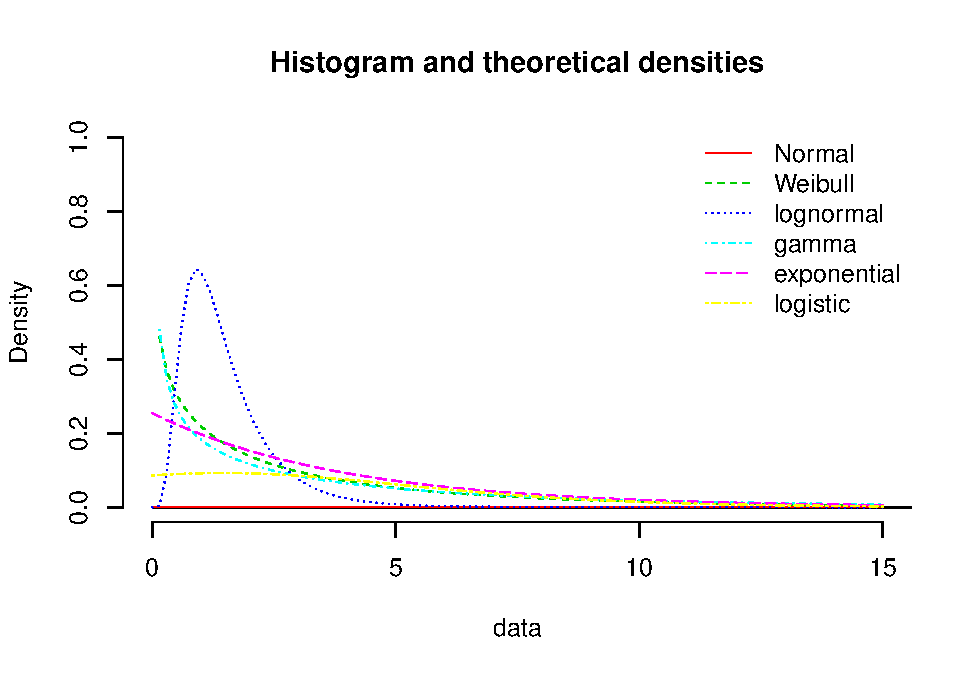
\includegraphics{analysis_files/figure-latex/unnamed-chunk-18-1.pdf}

\begin{Shaded}
\begin{Highlighting}[]
\KeywordTok{gofstat}\NormalTok{(}\KeywordTok{list}\NormalTok{(fit.sell.norm, fit.sell.weibull,fit.sell.lnorm,fit.sell.gamma,fit.sell.exp,fit.sell.logis),}\DataTypeTok{fitnames =} \KeywordTok{c}\NormalTok{(}\StringTok{"Normal"}\NormalTok{, }\StringTok{"Weibull"}\NormalTok{, }\StringTok{"Lognormal"}\NormalTok{, }\StringTok{"Gamma"}\NormalTok{, }\StringTok{"Exponential"}\NormalTok{, }\StringTok{"Logistic"}\NormalTok{))}
\end{Highlighting}
\end{Shaded}

\begin{verbatim}
## Goodness-of-fit statistics
##                                    Normal      Weibull    Lognormal
## Kolmogorov-Smirnov statistic 4.974599e-01 4.490602e-01    0.4613547
## Cramer-von Mises statistic   1.439686e+04 1.026181e+04 7993.0130687
## Anderson-Darling statistic            Inf          Inf          Inf
##                                     Gamma  Exponential     Logistic
## Kolmogorov-Smirnov statistic 4.366792e-01 5.729911e-01 4.578689e-01
## Cramer-von Mises statistic   1.057106e+04 1.638435e+04 1.007920e+04
## Anderson-Darling statistic            Inf          Inf          Inf
## 
## Goodness-of-fit criteria
##                                 Normal  Weibull Lognormal    Gamma
## Akaike's Information Criterion 2628308 641758.2  383593.2 772831.3
## Bayesian Information Criterion 2628328 641778.3  383613.4 772851.4
##                                Exponential Logistic
## Akaike's Information Criterion    824394.1  1158600
## Bayesian Information Criterion    824404.2  1158620
\end{verbatim}

\paragraph{From the goodness of fit statistics and the previous graph,
it seems lognormal is a better fit than the
rest}\label{from-the-goodness-of-fit-statistics-and-the-previous-graph-it-seems-lognormal-is-a-better-fit-than-the-rest}

\paragraph{Estimating parmaters for this
distribution}\label{estimating-parmaters-for-this-distribution-1}

\begin{Shaded}
\begin{Highlighting}[]
\NormalTok{fit.sell.lnorm}
\end{Highlighting}
\end{Shaded}

\begin{verbatim}
## Fitting of the distribution ' lnorm ' by maximum likelihood 
## Parameters:
##          estimate   Std. Error
## meanlog 0.2415419 0.0013709982
## sdlog   0.5719955 0.0009694288
\end{verbatim}

\begin{Shaded}
\begin{Highlighting}[]
\NormalTok{ests.sells <-}\StringTok{ }\KeywordTok{bootdist}\NormalTok{(fit.sell.lnorm, }\DataTypeTok{niter =} \DecValTok{100}\NormalTok{)}
\KeywordTok{summary}\NormalTok{(ests.sells)}
\end{Highlighting}
\end{Shaded}

\begin{verbatim}
## Parametric bootstrap medians and 95% percentile CI 
##            Median      2.5%     97.5%
## meanlog 0.2414480 0.2392662 0.2442888
## sdlog   0.5719517 0.5698143 0.5742834
\end{verbatim}

\subsection{\texorpdfstring{Analysis on token
`networkyocoinTX'}{Analysis on token networkyocoinTX}}\label{analysis-on-token-networkyocointx}

\paragraph{Loading token graph edge file into a
dataframe}\label{loading-token-graph-edge-file-into-a-dataframe-1}

\begin{Shaded}
\begin{Highlighting}[]
\NormalTok{networkyocoinTX <-}\StringTok{ }\KeywordTok{read.csv}\NormalTok{(}\StringTok{'data/networkyocoinTX.txt'}\NormalTok{, }\DataTypeTok{sep=}\StringTok{" "}\NormalTok{, }\DataTypeTok{header =} \OtherTok{FALSE}\NormalTok{)}
\KeywordTok{names}\NormalTok{(networkyocoinTX) <-}\StringTok{ }\KeywordTok{c}\NormalTok{(}\StringTok{"fromAddress"}\NormalTok{, }\StringTok{"toAddress"}\NormalTok{, }\StringTok{"unixTime"}\NormalTok{, }\StringTok{"tokenAmount"}\NormalTok{)}
\KeywordTok{head}\NormalTok{(networkyocoinTX)}
\end{Highlighting}
\end{Shaded}

\begin{verbatim}
##   fromAddress toAddress   unixTime tokenAmount
## 1     9911592   9911593 1517342415     5.0e+16
## 2     9911594   9911595 1517818943     1.0e+19
## 3     9911596   9911597 1515768296     5.0e+16
## 4     9911598   9911599 1512953126     1.3e+18
## 5     9911600   9911601 1512953651     8.0e+16
## 6     9911602   9911594 1512967870     1.0e+19
\end{verbatim}

\paragraph{Checking the data type for each
column}\label{checking-the-data-type-for-each-column-1}

\begin{Shaded}
\begin{Highlighting}[]
\KeywordTok{str}\NormalTok{(networkyocoinTX)}
\end{Highlighting}
\end{Shaded}

\begin{verbatim}
## 'data.frame':    746397 obs. of  4 variables:
##  $ fromAddress: int  9911592 9911594 9911596 9911598 9911600 9911602 9911598 9911603 9911605 9911606 ...
##  $ toAddress  : int  9911593 9911595 9911597 9911599 9911601 9911594 9911599 9911604 5496939 9911607 ...
##  $ unixTime   : int  1517342415 1517818943 1515768296 1512953126 1512953651 1512967870 1512971620 1513141671 1513607144 1513620522 ...
##  $ tokenAmount: num  5.0e+16 1.0e+19 5.0e+16 1.3e+18 8.0e+16 ...
\end{verbatim}

\paragraph{All columns have correct data types. We'll now check if there
are any transactions with same
addresses}\label{all-columns-have-correct-data-types.-well-now-check-if-there-are-any-transactions-with-same-addresses-1}

\begin{Shaded}
\begin{Highlighting}[]
\NormalTok{sameTxYocoin <-}\StringTok{ }\NormalTok{networkyocoinTX[networkyocoinTX}\OperatorTok{$}\NormalTok{fromAddress }\OperatorTok{==}\StringTok{ }\NormalTok{networkyocoinTX}\OperatorTok{$}\NormalTok{toAddress, ] }
\KeywordTok{nrow}\NormalTok{(sameTxYocoin)}
\end{Highlighting}
\end{Shaded}

\begin{verbatim}
## [1] 631
\end{verbatim}

\paragraph{It can be observed that there were 635 transactions that
occured where sender and recipient have the same
address.}\label{it-can-be-observed-that-there-were-635-transactions-that-occured-where-sender-and-recipient-have-the-same-address.-1}

\begin{Shaded}
\begin{Highlighting}[]
\KeywordTok{nrow}\NormalTok{(}\KeywordTok{unique}\NormalTok{(sameTxYocoin[}\StringTok{"fromAddress"}\NormalTok{]))}
\end{Highlighting}
\end{Shaded}

\begin{verbatim}
## [1] 4
\end{verbatim}

\paragraph{We observe that there are 4 unique addresses which have self
transactions.These are malicious user transactions and we'll remove them
from our
analysis.}\label{we-observe-that-there-are-4-unique-addresses-which-have-self-transactions.these-are-malicious-user-transactions-and-well-remove-them-from-our-analysis.}

\begin{Shaded}
\begin{Highlighting}[]
\NormalTok{cleanedYocoinTX <-}\StringTok{ }\NormalTok{networkyocoinTX[networkyocoinTX}\OperatorTok{$}\NormalTok{fromAddress }\OperatorTok{!=}\StringTok{ }\NormalTok{networkyocoinTX}\OperatorTok{$}\NormalTok{toAddress, ] }
\end{Highlighting}
\end{Shaded}

\paragraph{\texorpdfstring{Checking if any of the token amount exceeds
the total supply of the coin, which is limited to (554925923)
(\url{https://coinmarketcap.com/currencies/yocoin/})}{Checking if any of the token amount exceeds the total supply of the coin, which is limited to (554925923) (https://coinmarketcap.com/currencies/yocoin/)}}\label{checking-if-any-of-the-token-amount-exceeds-the-total-supply-of-the-coin-which-is-limited-to-554925923-httpscoinmarketcap.comcurrenciesyocoin}

\paragraph{Each coin can have upto a maximum of 10\^{}18 subunits.
Therefore, the token amount that can exist in the data should be less
than total supply * 10\^{}18. Anything beyond this amount will be
considered as outliers and removed from
analysis.}\label{each-coin-can-have-upto-a-maximum-of-1018-subunits.-therefore-the-token-amount-that-can-exist-in-the-data-should-be-less-than-total-supply-1018.-anything-beyond-this-amount-will-be-considered-as-outliers-and-removed-from-analysis.-1}

\begin{Shaded}
\begin{Highlighting}[]
\NormalTok{subUnits.yocoin <-}\StringTok{ }\DecValTok{10}\OperatorTok{^}\DecValTok{18}
\NormalTok{totalSupply.yocoin <-}\StringTok{ }\DecValTok{554925923}
\NormalTok{outliersDf.yocoin <-}\StringTok{ }\NormalTok{cleanedYocoinTX[cleanedYocoinTX}\OperatorTok{$}\NormalTok{tokenAmount }\OperatorTok{>}\StringTok{ }\NormalTok{totalSupply.yocoin }\OperatorTok{*}\StringTok{ }\NormalTok{subUnits.yocoin,]}
\KeywordTok{nrow}\NormalTok{(outliersDf.yocoin)}
\end{Highlighting}
\end{Shaded}

\begin{verbatim}
## [1] 90
\end{verbatim}

\paragraph{It can be observed that for 90 transactions, the token amount
is larger than the expected total supply of the coins. This anomaly can
be attributed to the BatchOverflow Exploit which resulted in generating
astronomical values. We'll remove such transaction from our
analysis.}\label{it-can-be-observed-that-for-90-transactions-the-token-amount-is-larger-than-the-expected-total-supply-of-the-coins.-this-anomaly-can-be-attributed-to-the-batchoverflow-exploit-which-resulted-in-generating-astronomical-values.-well-remove-such-transaction-from-our-analysis.}

\paragraph{\texorpdfstring{After removing the invalid transactions,
we'll generate the `buy' distribution. This will contain the frequency
of number of buys performed by
users}{After removing the invalid transactions, we'll generate the buy distribution. This will contain the frequency of number of buys performed by users}}\label{after-removing-the-invalid-transactions-well-generate-the-buy-distribution.-this-will-contain-the-frequency-of-number-of-buys-performed-by-users-1}

\begin{Shaded}
\begin{Highlighting}[]
\NormalTok{filteredYocoinTX <-}\StringTok{ }\NormalTok{cleanedYocoinTX[cleanedYocoinTX}\OperatorTok{$}\NormalTok{tokenAmount }\OperatorTok{<=}\StringTok{ }\NormalTok{totalSupply.yocoin }\OperatorTok{*}\StringTok{ }\NormalTok{subUnits.yocoin,]}
\CommentTok{#buys.distribution <- filteredGolemTX %>% group_by(toNode) %>% summarise(n = n()) %>% ungroup}
\NormalTok{yocoin.pair.users.buys <-}\StringTok{ }\NormalTok{filteredYocoinTX }\OperatorTok\StringTok{ }\KeywordTok{group_by}\NormalTok{(toAddress) }\OperatorTok\StringTok{ }\KeywordTok{summarise}\NormalTok{(}\DataTypeTok{n =} \KeywordTok{n}\NormalTok{(), }\DataTypeTok{sumAmount=}\KeywordTok{sum}\NormalTok{(tokenAmount)) }\OperatorTok\StringTok{ }\NormalTok{ungroup}
\KeywordTok{head}\NormalTok{(yocoin.pair.users.buys)}
\end{Highlighting}
\end{Shaded}

\begin{verbatim}
## # A tibble: 6 x 3
##   toAddress     n sumAmount
##       <int> <int>     <dbl>
## 1     14514     1   4.93e19
## 2     16853     3   2.98e18
## 3     29745     3   4.33e22
## 4     48730     1   2.23e17
## 5    104010     1   1.00e18
## 6    186374     1   1.82e16
\end{verbatim}

\subsubsection{\texorpdfstring{Plotting density distribution for `Buy'
transactions. We'll check if we are able to identify frequency of number
of buys between 2
users}{Plotting density distribution for Buy transactions. We'll check if we are able to identify frequency of number of buys between 2 users}}\label{plotting-density-distribution-for-buy-transactions.-well-check-if-we-are-able-to-identify-frequency-of-number-of-buys-between-2-users-1}

\begin{Shaded}
\begin{Highlighting}[]
\KeywordTok{ggplot}\NormalTok{(}\DataTypeTok{data=}\NormalTok{yocoin.pair.users.buys, }\KeywordTok{aes}\NormalTok{(yocoin.pair.users.buys}\OperatorTok{$}\NormalTok{n)) }\OperatorTok{+}\StringTok{ }
\StringTok{  }\KeywordTok{geom_density}\NormalTok{(}\DataTypeTok{fill=}\StringTok{'yellow'}\NormalTok{, }\DataTypeTok{color=}\StringTok{'yellow'}\NormalTok{) }\OperatorTok{+}\StringTok{ }
\StringTok{  }\KeywordTok{scale_x_continuous}\NormalTok{(}\DataTypeTok{breaks=}\KeywordTok{seq}\NormalTok{(}\DecValTok{0}\NormalTok{,}\DecValTok{160}\NormalTok{,}\DecValTok{20}\NormalTok{), }\DataTypeTok{limits=}\KeywordTok{c}\NormalTok{(}\DecValTok{0}\NormalTok{,}\DecValTok{160}\NormalTok{)) }\OperatorTok{+}\StringTok{ }
\StringTok{  }\KeywordTok{xlab}\NormalTok{(}\StringTok{"No. of buys (Pair-wise)"}\NormalTok{) }\OperatorTok{+}
\StringTok{  }\KeywordTok{ylab}\NormalTok{(}\StringTok{"Density"}\NormalTok{) }\OperatorTok{+}\StringTok{ }
\StringTok{  }\KeywordTok{ggtitle}\NormalTok{(}\StringTok{"Buy Distribution"}\NormalTok{) }\OperatorTok{+}
\StringTok{  }\KeywordTok{theme}\NormalTok{(}\DataTypeTok{text =} \KeywordTok{element_text}\NormalTok{(}\DataTypeTok{color =} \StringTok{"#444444"}\NormalTok{)}
\NormalTok{        ,}\DataTypeTok{panel.background =} \KeywordTok{element_rect}\NormalTok{(}\DataTypeTok{fill =} \StringTok{'#444B5A'}\NormalTok{)}
\NormalTok{        ,}\DataTypeTok{panel.grid.minor =} \KeywordTok{element_line}\NormalTok{(}\DataTypeTok{color =} \StringTok{'#4d5566'}\NormalTok{)}
\NormalTok{        ,}\DataTypeTok{panel.grid.major =} \KeywordTok{element_line}\NormalTok{(}\DataTypeTok{color =} \StringTok{'#586174'}\NormalTok{)}
\NormalTok{        ,}\DataTypeTok{plot.title =} \KeywordTok{element_text}\NormalTok{(}\DataTypeTok{size =} \DecValTok{24}\NormalTok{)}
\NormalTok{        ,}\DataTypeTok{axis.title =} \KeywordTok{element_text}\NormalTok{(}\DataTypeTok{size =} \DecValTok{18}\NormalTok{, }\DataTypeTok{color =} \StringTok{'#555555'}\NormalTok{)}
\NormalTok{        ,}\DataTypeTok{axis.title.y =} \KeywordTok{element_text}\NormalTok{(}\DataTypeTok{vjust =}\NormalTok{ .}\DecValTok{5}\NormalTok{, }\DataTypeTok{angle =} \DecValTok{0}\NormalTok{)}
\NormalTok{        ,}\DataTypeTok{axis.title.x =} \KeywordTok{element_text}\NormalTok{(}\DataTypeTok{hjust =}\NormalTok{ .}\DecValTok{5}\NormalTok{)}
\NormalTok{  ) }
\end{Highlighting}
\end{Shaded}

\begin{verbatim}
## Warning: Removed 970 rows containing non-finite values (stat_density).
\end{verbatim}

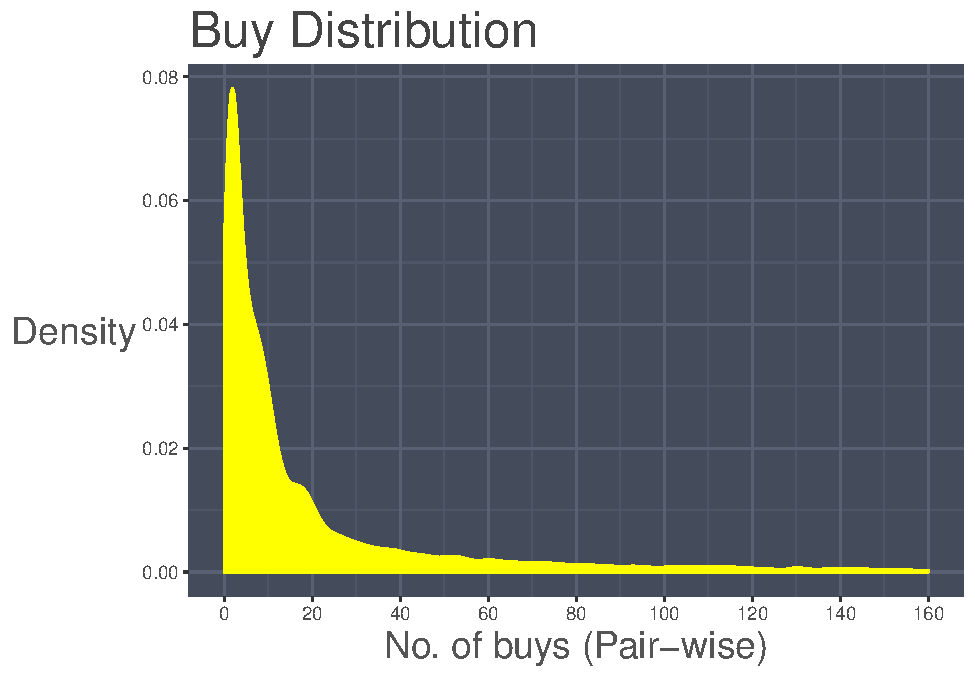
\includegraphics{analysis_files/figure-latex/unnamed-chunk-29-1.pdf}
\#\#\#Similarly, we'll generate the `sell' distribution. This will
contain the frequency of number of sells performed by users

\begin{Shaded}
\begin{Highlighting}[]
\NormalTok{yocoin.pair.users.sells <-}\StringTok{ }\NormalTok{filteredYocoinTX }\OperatorTok\StringTok{ }\KeywordTok{group_by}\NormalTok{(fromAddress) }\OperatorTok\StringTok{ }\KeywordTok{summarise}\NormalTok{(}\DataTypeTok{n =} \KeywordTok{n}\NormalTok{(), }\DataTypeTok{sumAmount=}\KeywordTok{sum}\NormalTok{(tokenAmount))}
\KeywordTok{head}\NormalTok{(yocoin.pair.users.sells)}
\end{Highlighting}
\end{Shaded}

\begin{verbatim}
## # A tibble: 6 x 3
##   fromAddress     n sumAmount
##         <int> <int>     <dbl>
## 1      309659  4103   1.01e24
## 2      336069   133   2.98e22
## 3      467727     3   9.00e19
## 4      483085    64   7.85e21
## 5     1380386     2   2.88e20
## 6     1387470     2   8.97e20
\end{verbatim}

\paragraph{\texorpdfstring{Plotting density distribution for `Sell'
transactions}{Plotting density distribution for Sell transactions}}\label{plotting-density-distribution-for-sell-transactions-1}

\begin{Shaded}
\begin{Highlighting}[]
\KeywordTok{ggplot}\NormalTok{(}\DataTypeTok{data=}\NormalTok{yocoin.pair.users.sells, }\KeywordTok{aes}\NormalTok{(yocoin.pair.users.sells}\OperatorTok{$}\NormalTok{n)) }\OperatorTok{+}\StringTok{ }
\StringTok{  }\KeywordTok{geom_density}\NormalTok{(}\DataTypeTok{fill=}\StringTok{'cyan'}\NormalTok{, }\DataTypeTok{color=}\StringTok{'cyan'}\NormalTok{) }\OperatorTok{+}\StringTok{ }
\StringTok{  }\KeywordTok{scale_x_continuous}\NormalTok{(}\DataTypeTok{breaks=}\KeywordTok{seq}\NormalTok{(}\DecValTok{0}\NormalTok{,}\DecValTok{20}\NormalTok{,}\DecValTok{1}\NormalTok{), }\DataTypeTok{limits=}\KeywordTok{c}\NormalTok{(}\DecValTok{0}\NormalTok{,}\DecValTok{20}\NormalTok{)) }\OperatorTok{+}\StringTok{ }
\StringTok{  }\KeywordTok{xlab}\NormalTok{(}\StringTok{"No. of sells (Pair-wise)"}\NormalTok{) }\OperatorTok{+}
\StringTok{  }\KeywordTok{ylab}\NormalTok{(}\StringTok{"Density"}\NormalTok{) }\OperatorTok{+}\StringTok{ }
\StringTok{  }\KeywordTok{ggtitle}\NormalTok{(}\StringTok{"Sell Distribution"}\NormalTok{) }\OperatorTok{+}\StringTok{ }
\StringTok{  }\KeywordTok{theme}\NormalTok{(}\DataTypeTok{text =} \KeywordTok{element_text}\NormalTok{(}\DataTypeTok{color =} \StringTok{"#444444"}\NormalTok{)}
\NormalTok{        ,}\DataTypeTok{panel.background =} \KeywordTok{element_rect}\NormalTok{(}\DataTypeTok{fill =} \StringTok{'#444B5A'}\NormalTok{)}
\NormalTok{        ,}\DataTypeTok{panel.grid.minor =} \KeywordTok{element_line}\NormalTok{(}\DataTypeTok{color =} \StringTok{'#4d5566'}\NormalTok{)}
\NormalTok{        ,}\DataTypeTok{panel.grid.major =} \KeywordTok{element_line}\NormalTok{(}\DataTypeTok{color =} \StringTok{'#586174'}\NormalTok{)}
\NormalTok{        ,}\DataTypeTok{plot.title =} \KeywordTok{element_text}\NormalTok{(}\DataTypeTok{size =} \DecValTok{24}\NormalTok{)}
\NormalTok{        ,}\DataTypeTok{axis.title =} \KeywordTok{element_text}\NormalTok{(}\DataTypeTok{size =} \DecValTok{18}\NormalTok{, }\DataTypeTok{color =} \StringTok{'#555555'}\NormalTok{)}
\NormalTok{        ,}\DataTypeTok{axis.title.y =} \KeywordTok{element_text}\NormalTok{(}\DataTypeTok{vjust =}\NormalTok{ .}\DecValTok{5}\NormalTok{, }\DataTypeTok{angle =} \DecValTok{0}\NormalTok{)}
\NormalTok{        ,}\DataTypeTok{axis.title.x =} \KeywordTok{element_text}\NormalTok{(}\DataTypeTok{hjust =}\NormalTok{ .}\DecValTok{5}\NormalTok{)}
\NormalTok{  )}
\end{Highlighting}
\end{Shaded}

\begin{verbatim}
## Warning: Removed 263 rows containing non-finite values (stat_density).
\end{verbatim}

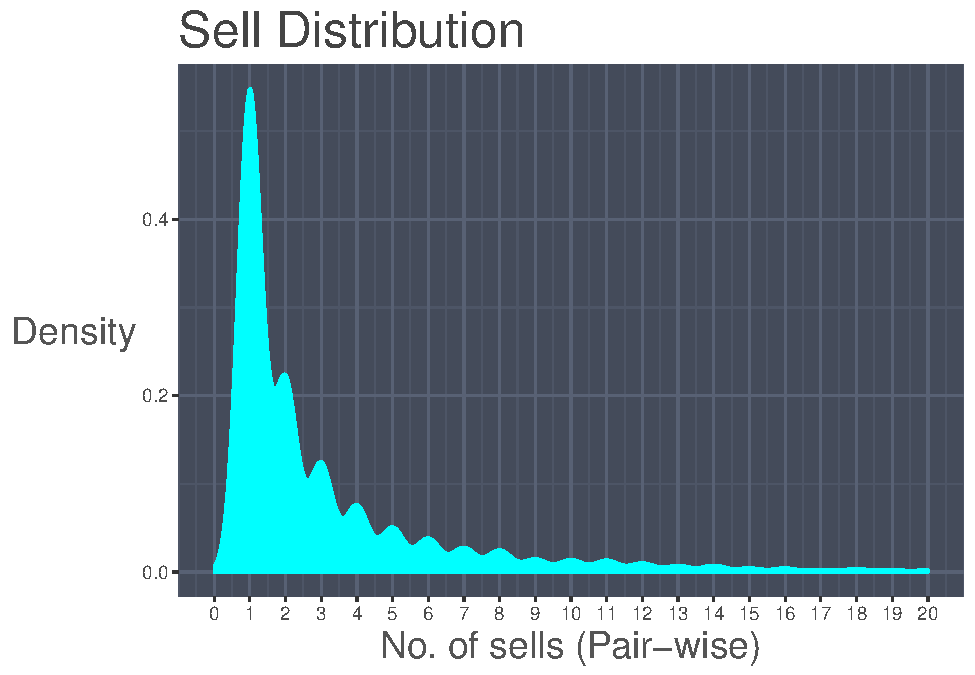
\includegraphics{analysis_files/figure-latex/unnamed-chunk-31-1.pdf}
\#\#\#Now that we have seen density distributions for both types of
transactions, we'll individually fit the data in different distribution
models

\begin{Shaded}
\begin{Highlighting}[]
\NormalTok{yocoin.fit.buy.norm <-}\StringTok{ }\KeywordTok{fitdist}\NormalTok{(yocoin.pair.users.buys}\OperatorTok{$}\NormalTok{n, }\StringTok{"norm"}\NormalTok{)}
\NormalTok{yocoin.fit.buy.weibull <-}\StringTok{ }\KeywordTok{fitdist}\NormalTok{(yocoin.pair.users.buys}\OperatorTok{$}\NormalTok{n, }\StringTok{"weibull"}\NormalTok{)}
\NormalTok{yocoin.fit.buy.gamma <-}\StringTok{ }\KeywordTok{fitdist}\NormalTok{(yocoin.pair.users.buys}\OperatorTok{$}\NormalTok{n, }\StringTok{"gamma"}\NormalTok{)}
\NormalTok{yocoin.fit.buy.lnorm <-}\StringTok{ }\KeywordTok{fitdist}\NormalTok{(yocoin.pair.users.buys}\OperatorTok{$}\NormalTok{n, }\StringTok{"lnorm"}\NormalTok{)}
\NormalTok{yocoin.fit.buy.exp <-}\StringTok{ }\KeywordTok{fitdist}\NormalTok{(yocoin.pair.users.buys}\OperatorTok{$}\NormalTok{n, }\StringTok{"exp"}\NormalTok{)}
\NormalTok{yocoin.fit.buy.logis <-}\StringTok{ }\KeywordTok{fitdist}\NormalTok{(yocoin.pair.users.buys}\OperatorTok{$}\NormalTok{n, }\StringTok{"logis"}\NormalTok{)}
\end{Highlighting}
\end{Shaded}

\paragraph{\texorpdfstring{Plotting all distributions and check which
one satisfies our `Buy'
distribution}{Plotting all distributions and check which one satisfies our Buy distribution}}\label{plotting-all-distributions-and-check-which-one-satisfies-our-buy-distribution-1}

\begin{Shaded}
\begin{Highlighting}[]
\NormalTok{plot.legend <-}\StringTok{ }\KeywordTok{c}\NormalTok{(}\StringTok{"Normal"}\NormalTok{, }\StringTok{"Weibull"}\NormalTok{, }\StringTok{"lognormal"}\NormalTok{, }\StringTok{"gamma"}\NormalTok{, }\StringTok{"exponential"}\NormalTok{, }\StringTok{"logistic"}\NormalTok{)}
\KeywordTok{denscomp}\NormalTok{(}\KeywordTok{list}\NormalTok{(yocoin.fit.buy.norm,yocoin.fit.buy.weibull , yocoin.fit.buy.lnorm, yocoin.fit.buy.gamma, yocoin.fit.buy.exp,yocoin.fit.buy.logis), }\DataTypeTok{legendtext =}\NormalTok{ plot.legend, }\DataTypeTok{xlim=}\KeywordTok{c}\NormalTok{(}\DecValTok{0}\NormalTok{,}\DecValTok{160}\NormalTok{), }\DataTypeTok{ylim=}\KeywordTok{c}\NormalTok{(}\DecValTok{0}\NormalTok{,}\FloatTok{0.1}\NormalTok{))}
\end{Highlighting}
\end{Shaded}

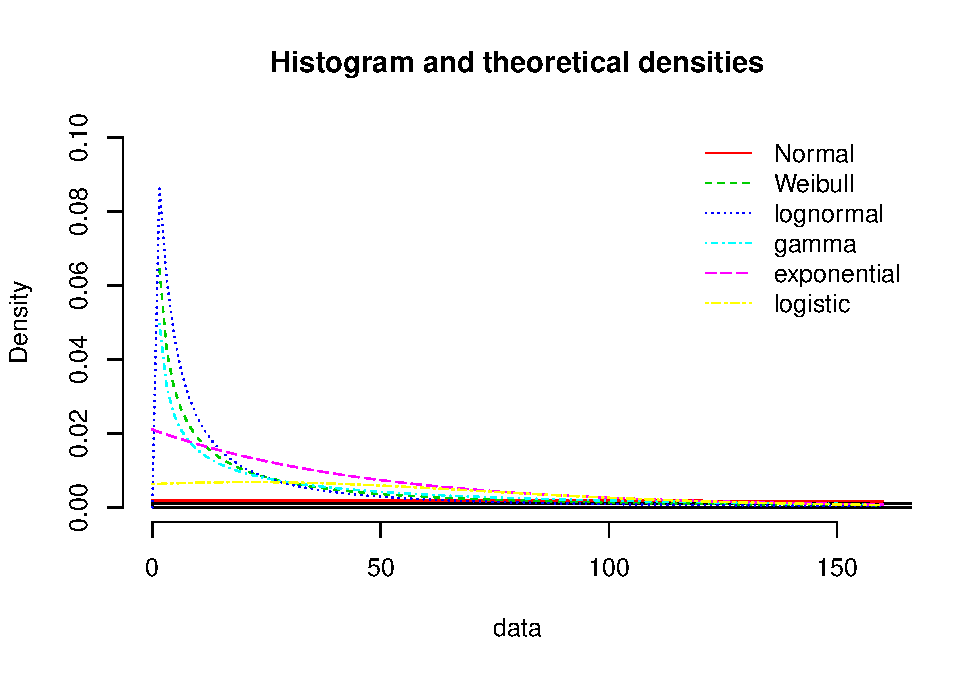
\includegraphics{analysis_files/figure-latex/unnamed-chunk-33-1.pdf}

\begin{Shaded}
\begin{Highlighting}[]
\KeywordTok{gofstat}\NormalTok{(}\KeywordTok{list}\NormalTok{(yocoin.fit.buy.norm,yocoin.fit.buy.weibull , yocoin.fit.buy.lnorm, yocoin.fit.buy.gamma, yocoin.fit.buy.exp,yocoin.fit.buy.logis),}\DataTypeTok{fitnames =} \KeywordTok{c}\NormalTok{(}\StringTok{"Normal"}\NormalTok{, }\StringTok{"Weibull"}\NormalTok{, }\StringTok{"Lognormal"}\NormalTok{, }\StringTok{"Gamma"}\NormalTok{, }\StringTok{"Exponential"}\NormalTok{, }\StringTok{"Logistic"}\NormalTok{))}
\end{Highlighting}
\end{Shaded}

\begin{verbatim}
## Goodness-of-fit statistics
##                                   Normal     Weibull   Lognormal
## Kolmogorov-Smirnov statistic   0.4146914   0.1670572   0.0910452
## Cramer-von Mises statistic   837.2258143  66.7021970  17.5966375
## Anderson-Darling statistic           Inf 449.2154012 161.2311097
##                                    Gamma  Exponential    Logistic
## Kolmogorov-Smirnov statistic   0.1901254    0.3901345   0.3646005
## Cramer-von Mises statistic   195.6824678 1006.9359569 453.2672980
## Anderson-Darling statistic           Inf          Inf         Inf
## 
## Goodness-of-fit criteria
##                                  Normal  Weibull Lognormal    Gamma
## Akaike's Information Criterion 213088.5 134580.6  129937.9 139184.7
## Bayesian Information Criterion 213103.8 134595.9  129953.2 139200.0
##                                Exponential Logistic
## Akaike's Information Criterion    152479.1 182363.4
## Bayesian Information Criterion    152486.7 182378.7
\end{verbatim}

\paragraph{From the goodness of fit statistics and the previous graph,
it seems lognormal is a better fit than the
rest.}\label{from-the-goodness-of-fit-statistics-and-the-previous-graph-it-seems-lognormal-is-a-better-fit-than-the-rest.-1}

\paragraph{Estimating parmaters for this
distribution}\label{estimating-parmaters-for-this-distribution-2}

\begin{Shaded}
\begin{Highlighting}[]
\NormalTok{yocoin.fit.buy.lnorm}
\end{Highlighting}
\end{Shaded}

\begin{verbatim}
## Fitting of the distribution ' lnorm ' by maximum likelihood 
## Parameters:
##         estimate  Std. Error
## meanlog 2.216576 0.013265610
## sdlog   1.661170 0.009380187
\end{verbatim}

\begin{Shaded}
\begin{Highlighting}[]
\NormalTok{yocoin.ests.buys <-}\StringTok{ }\KeywordTok{bootdist}\NormalTok{(yocoin.fit.buy.lnorm, }\DataTypeTok{niter =} \DecValTok{1000}\NormalTok{)}
\KeywordTok{summary}\NormalTok{(yocoin.ests.buys)}
\end{Highlighting}
\end{Shaded}

\begin{verbatim}
## Parametric bootstrap medians and 95% percentile CI 
##           Median     2.5%    97.5%
## meanlog 2.216219 2.191376 2.242184
## sdlog   1.661220 1.642817 1.680019
\end{verbatim}

\paragraph{Now fitting distributions for sell
transactions.}\label{now-fitting-distributions-for-sell-transactions.}

\begin{Shaded}
\begin{Highlighting}[]
\NormalTok{yocoin.fit.sell.norm <-}\StringTok{ }\KeywordTok{fitdist}\NormalTok{(yocoin.pair.users.sells}\OperatorTok{$}\NormalTok{n, }\StringTok{"norm"}\NormalTok{)}
\NormalTok{yocoin.fit.sell.weibull <-}\StringTok{ }\KeywordTok{fitdist}\NormalTok{(yocoin.pair.users.sells}\OperatorTok{$}\NormalTok{n, }\StringTok{"weibull"}\NormalTok{)}
\NormalTok{yocoin.fit.sell.gamma <-}\StringTok{ }\KeywordTok{fitdist}\NormalTok{(yocoin.pair.users.sells}\OperatorTok{$}\NormalTok{n, }\StringTok{"gamma"}\NormalTok{)}
\NormalTok{yocoin.fit.sell.lnorm <-}\StringTok{ }\KeywordTok{fitdist}\NormalTok{(yocoin.pair.users.sells}\OperatorTok{$}\NormalTok{n, }\StringTok{"lnorm"}\NormalTok{)}
\NormalTok{yocoin.fit.sell.exp <-}\StringTok{ }\KeywordTok{fitdist}\NormalTok{(yocoin.pair.users.sells}\OperatorTok{$}\NormalTok{n, }\StringTok{"exp"}\NormalTok{)}
\NormalTok{yocoin.fit.sell.logis <-}\StringTok{ }\KeywordTok{fitdist}\NormalTok{(yocoin.pair.users.sells}\OperatorTok{$}\NormalTok{n, }\StringTok{"logis"}\NormalTok{)}
\end{Highlighting}
\end{Shaded}

\subsubsection{\texorpdfstring{Plotting all distributions and check
which one satisfies our `Sell'
distribution}{Plotting all distributions and check which one satisfies our Sell distribution}}\label{plotting-all-distributions-and-check-which-one-satisfies-our-sell-distribution-1}

\begin{Shaded}
\begin{Highlighting}[]
\NormalTok{plot.legend <-}\StringTok{ }\KeywordTok{c}\NormalTok{(}\StringTok{"Normal"}\NormalTok{,}\StringTok{"Weibull"}\NormalTok{, }\StringTok{"lognormal"}\NormalTok{, }\StringTok{"gamma"}\NormalTok{, }\StringTok{"exponential"}\NormalTok{, }\StringTok{"logistic"}\NormalTok{)}
\KeywordTok{denscomp}\NormalTok{(}\KeywordTok{list}\NormalTok{(yocoin.fit.sell.norm, yocoin.fit.sell.weibull, yocoin.fit.sell.lnorm, yocoin.fit.sell.gamma, yocoin.fit.sell.exp,yocoin.fit.sell.logis),}\DataTypeTok{plotstyle =} \StringTok{"graphics"}\NormalTok{, }\DataTypeTok{legendtext =}\NormalTok{ plot.legend, }\DataTypeTok{xlim=}\KeywordTok{c}\NormalTok{(}\DecValTok{0}\NormalTok{,}\DecValTok{15}\NormalTok{), }\DataTypeTok{ylim=}\KeywordTok{c}\NormalTok{(}\DecValTok{0}\NormalTok{,}\FloatTok{0.6}\NormalTok{)) }
\end{Highlighting}
\end{Shaded}

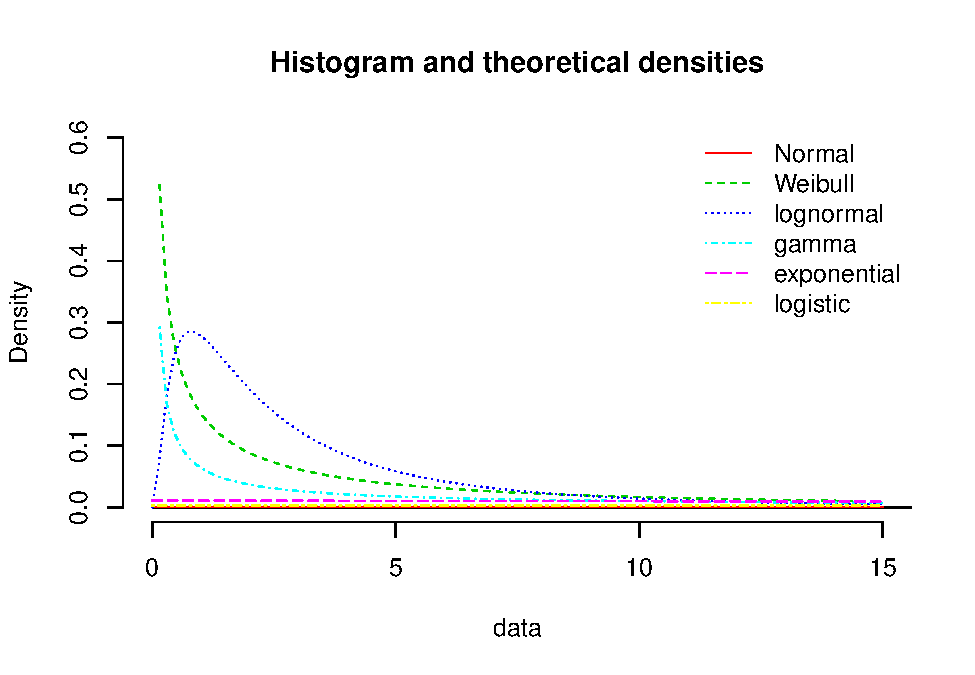
\includegraphics{analysis_files/figure-latex/unnamed-chunk-38-1.pdf}

\begin{Shaded}
\begin{Highlighting}[]
\KeywordTok{gofstat}\NormalTok{(}\KeywordTok{list}\NormalTok{(yocoin.fit.sell.norm, yocoin.fit.sell.weibull, yocoin.fit.sell.lnorm, yocoin.fit.sell.gamma, yocoin.fit.sell.exp,yocoin.fit.sell.logis),}\DataTypeTok{fitnames =} \KeywordTok{c}\NormalTok{(}\StringTok{"Normal"}\NormalTok{, }\StringTok{"Weibull"}\NormalTok{, }\StringTok{"Lognormal"}\NormalTok{, }\StringTok{"Gamma"}\NormalTok{, }\StringTok{"Exponential"}\NormalTok{, }\StringTok{"Logistic"}\NormalTok{))}
\end{Highlighting}
\end{Shaded}

\begin{verbatim}
## Goodness-of-fit statistics
##                                   Normal    Weibull  Lognormal       Gamma
## Kolmogorov-Smirnov statistic   0.4948287   0.386072  0.2355341   0.4142792
## Cramer-von Mises statistic   673.4024818 201.825519 81.2617214 508.9603200
## Anderson-Darling statistic           Inf        Inf        Inf         Inf
##                              Exponential    Logistic
## Kolmogorov-Smirnov statistic    0.815979   0.4892786
## Cramer-von Mises statistic   2214.196711 619.0460399
## Anderson-Darling statistic           Inf         Inf
## 
## Goodness-of-fit criteria
##                                  Normal  Weibull Lognormal    Gamma
## Akaike's Information Criterion 164061.2 45681.33  37189.82 58866.71
## Bayesian Information Criterion 164075.2 45695.34  37203.83 58880.72
##                                Exponential Logistic
## Akaike's Information Criterion    89799.81 111560.8
## Bayesian Information Criterion    89806.81 111574.8
\end{verbatim}

\paragraph{From the goodness of fit statistics and the previous graph,
it seems lognormal is a better fit than the
rest}\label{from-the-goodness-of-fit-statistics-and-the-previous-graph-it-seems-lognormal-is-a-better-fit-than-the-rest-1}

\paragraph{Estimating parmaters for this
distribution}\label{estimating-parmaters-for-this-distribution-3}

\begin{Shaded}
\begin{Highlighting}[]
\NormalTok{yocoin.fit.sell.lnorm}
\end{Highlighting}
\end{Shaded}

\begin{verbatim}
## Fitting of the distribution ' lnorm ' by maximum likelihood 
## Parameters:
##          estimate  Std. Error
## meanlog 0.8343167 0.011443193
## sdlog   1.0322369 0.008091525
\end{verbatim}

\begin{Shaded}
\begin{Highlighting}[]
\NormalTok{yocoin.ests.sells <-}\StringTok{ }\KeywordTok{bootdist}\NormalTok{(yocoin.fit.sell.lnorm, }\DataTypeTok{niter =} \DecValTok{100}\NormalTok{)}
\KeywordTok{summary}\NormalTok{(yocoin.ests.sells)}
\end{Highlighting}
\end{Shaded}

\begin{verbatim}
## Parametric bootstrap medians and 95% percentile CI 
##            Median     2.5%    97.5%
## meanlog 0.8363467 0.815102 0.858700
## sdlog   1.0309188 1.014825 1.046302
\end{verbatim}

\subsection{\texorpdfstring{Analysis on token
`networkomisegoTX'}{Analysis on token networkomisegoTX}}\label{analysis-on-token-networkomisegotx}

\paragraph{Loading token graph edge file into a
dataframe}\label{loading-token-graph-edge-file-into-a-dataframe-2}

\begin{Shaded}
\begin{Highlighting}[]
\NormalTok{networkomisegoTX <-}\StringTok{ }\KeywordTok{read.csv}\NormalTok{(}\StringTok{'data/networkomisegoTX.txt'}\NormalTok{, }\DataTypeTok{sep=}\StringTok{" "}\NormalTok{, }\DataTypeTok{header =} \OtherTok{FALSE}\NormalTok{)}
\KeywordTok{names}\NormalTok{(networkomisegoTX) <-}\StringTok{ }\KeywordTok{c}\NormalTok{(}\StringTok{"fromAddress"}\NormalTok{, }\StringTok{"toAddress"}\NormalTok{, }\StringTok{"unixTime"}\NormalTok{, }\StringTok{"tokenAmount"}\NormalTok{)}
\KeywordTok{head}\NormalTok{(networkomisegoTX)}
\end{Highlighting}
\end{Shaded}

\begin{verbatim}
##   fromAddress toAddress   unixTime  tokenAmount
## 1     5186357     75994 1524611290 2.465000e+19
## 2          13    168381 1524611320 1.700000e+21
## 3      142341     75994 1524611536 5.301102e+21
## 4     5186358    297278 1524611536 2.992292e+19
## 5     5186359    297278 1524611536 2.214251e+18
## 6     5186360    297278 1524611536 2.166550e+19
\end{verbatim}

\paragraph{We'll now check if there are any transactions with same
addresses}\label{well-now-check-if-there-are-any-transactions-with-same-addresses}

\begin{Shaded}
\begin{Highlighting}[]
\NormalTok{sameTxomisegoTX <-}\StringTok{ }\NormalTok{networkomisegoTX[networkomisegoTX}\OperatorTok{$}\NormalTok{fromAddress }\OperatorTok{==}\StringTok{ }\NormalTok{networkomisegoTX}\OperatorTok{$}\NormalTok{toAddress, ] }
\KeywordTok{nrow}\NormalTok{(sameTxomisegoTX)}
\end{Highlighting}
\end{Shaded}

\begin{verbatim}
## [1] 30347
\end{verbatim}

\paragraph{It can be observed that there were 30347 transactions that
occured where sender and recipient have the same
address}\label{it-can-be-observed-that-there-were-30347-transactions-that-occured-where-sender-and-recipient-have-the-same-address}

\begin{Shaded}
\begin{Highlighting}[]
\KeywordTok{nrow}\NormalTok{(}\KeywordTok{unique}\NormalTok{(sameTxomisegoTX[}\StringTok{"fromAddress"}\NormalTok{]))}
\end{Highlighting}
\end{Shaded}

\begin{verbatim}
## [1] 259
\end{verbatim}

\paragraph{We observe that there are 259 unique addresses which have
self transactions.These are malicious user transactions and we'll remove
them from our
analysis}\label{we-observe-that-there-are-259-unique-addresses-which-have-self-transactions.these-are-malicious-user-transactions-and-well-remove-them-from-our-analysis}

\begin{Shaded}
\begin{Highlighting}[]
\NormalTok{cleanedOmisegoTX <-}\StringTok{ }\NormalTok{networkomisegoTX[networkomisegoTX}\OperatorTok{$}\NormalTok{fromAddress }\OperatorTok{!=}\StringTok{ }\NormalTok{networkomisegoTX}\OperatorTok{$}\NormalTok{toAddress, ] }
\end{Highlighting}
\end{Shaded}

\paragraph{\texorpdfstring{Checking if any of the token amount exceeds
the total supply of the coin, which is limited to 140,245,398
(\url{https://coinmarketcap.com/currencies/omisego/})}{Checking if any of the token amount exceeds the total supply of the coin, which is limited to 140,245,398 (https://coinmarketcap.com/currencies/omisego/)}}\label{checking-if-any-of-the-token-amount-exceeds-the-total-supply-of-the-coin-which-is-limited-to-140245398-httpscoinmarketcap.comcurrenciesomisego}

\paragraph{Each coin can have upto a maximum of 10\^{}18 subunits.
Therefore, the token amount that can exist in the data should be less
than total supply * 10\^{}18. Anything beyond this amount will be
considered as outliers and removed from
analysis.}\label{each-coin-can-have-upto-a-maximum-of-1018-subunits.-therefore-the-token-amount-that-can-exist-in-the-data-should-be-less-than-total-supply-1018.-anything-beyond-this-amount-will-be-considered-as-outliers-and-removed-from-analysis.-2}

\begin{Shaded}
\begin{Highlighting}[]
\NormalTok{subUnits.omisego <-}\StringTok{ }\DecValTok{10}\OperatorTok{^}\DecValTok{18}
\NormalTok{totalSupply.omisego <-}\StringTok{ }\DecValTok{140245398}
\NormalTok{outliersDf.omisego <-}\StringTok{ }\NormalTok{cleanedOmisegoTX[cleanedOmisegoTX}\OperatorTok{$}\NormalTok{tokenAmount }\OperatorTok{>}\StringTok{ }\NormalTok{totalSupply.omisego }\OperatorTok{*}\StringTok{ }\NormalTok{subUnits.omisego,]}
\KeywordTok{nrow}\NormalTok{(outliersDf.omisego)}
\end{Highlighting}
\end{Shaded}

\begin{verbatim}
## [1] 10
\end{verbatim}

\paragraph{It can be observed that for 10 transactions, the token amount
is larger than the expected total supply of the coins. This anomaly can
be attributed to the BatchOverflow Exploit which resulted in generating
astronomical values. We'll remove such transaction from our
analysis.}\label{it-can-be-observed-that-for-10-transactions-the-token-amount-is-larger-than-the-expected-total-supply-of-the-coins.-this-anomaly-can-be-attributed-to-the-batchoverflow-exploit-which-resulted-in-generating-astronomical-values.-well-remove-such-transaction-from-our-analysis.}

\paragraph{\texorpdfstring{After removing the invalid transactions,
we'll generate the `buy' distribution. This will contain the frequency
of number of buys performed by
users}{After removing the invalid transactions, we'll generate the buy distribution. This will contain the frequency of number of buys performed by users}}\label{after-removing-the-invalid-transactions-well-generate-the-buy-distribution.-this-will-contain-the-frequency-of-number-of-buys-performed-by-users-2}

\begin{Shaded}
\begin{Highlighting}[]
\NormalTok{filteredOmisegoTX <-}\StringTok{ }\NormalTok{cleanedOmisegoTX[cleanedOmisegoTX}\OperatorTok{$}\NormalTok{tokenAmount }\OperatorTok{<=}\StringTok{ }\NormalTok{totalSupply.omisego }\OperatorTok{*}\StringTok{ }\NormalTok{subUnits.omisego,]}
\NormalTok{omisego.pair.users.buys <-}\StringTok{ }\NormalTok{filteredOmisegoTX }\OperatorTok\StringTok{ }\KeywordTok{group_by}\NormalTok{(toAddress) }\OperatorTok\StringTok{ }\KeywordTok{summarise}\NormalTok{(}\DataTypeTok{n =} \KeywordTok{n}\NormalTok{(), }\DataTypeTok{sumAmount=}\KeywordTok{sum}\NormalTok{(tokenAmount)) }\OperatorTok\StringTok{ }\NormalTok{ungroup}
\KeywordTok{head}\NormalTok{(omisego.pair.users.buys)}
\end{Highlighting}
\end{Shaded}

\begin{verbatim}
## # A tibble: 6 x 3
##   toAddress     n sumAmount
##       <int> <int>     <dbl>
## 1         0     1   4.00e19
## 2         1     1   4.00e19
## 3         2     2   7.91e19
## 4         3     1   9.00e18
## 5         4   132   3.46e22
## 6         5 57315   5.23e25
\end{verbatim}

\subsubsection{\texorpdfstring{Plotting density distribution for `Buy'
transactions. We'll check if we are able to identify frequency of number
of buys between 2
users}{Plotting density distribution for Buy transactions. We'll check if we are able to identify frequency of number of buys between 2 users}}\label{plotting-density-distribution-for-buy-transactions.-well-check-if-we-are-able-to-identify-frequency-of-number-of-buys-between-2-users-2}

\begin{Shaded}
\begin{Highlighting}[]
\KeywordTok{ggplot}\NormalTok{(}\DataTypeTok{data=}\NormalTok{omisego.pair.users.buys, }\KeywordTok{aes}\NormalTok{(omisego.pair.users.buys}\OperatorTok{$}\NormalTok{n)) }\OperatorTok{+}\StringTok{ }
\StringTok{  }\KeywordTok{geom_density}\NormalTok{(}\DataTypeTok{fill=}\StringTok{'yellow'}\NormalTok{, }\DataTypeTok{color=}\StringTok{'yellow'}\NormalTok{) }\OperatorTok{+}\StringTok{ }
\StringTok{  }\KeywordTok{scale_x_continuous}\NormalTok{(}\DataTypeTok{breaks=}\KeywordTok{seq}\NormalTok{(}\DecValTok{0}\NormalTok{,}\DecValTok{10}\NormalTok{,}\DecValTok{1}\NormalTok{), }\DataTypeTok{limits=}\KeywordTok{c}\NormalTok{(}\DecValTok{0}\NormalTok{,}\DecValTok{10}\NormalTok{)) }\OperatorTok{+}\StringTok{ }
\StringTok{  }\KeywordTok{xlab}\NormalTok{(}\StringTok{"No. of buys (Pair-wise)"}\NormalTok{) }\OperatorTok{+}
\StringTok{  }\KeywordTok{ylab}\NormalTok{(}\StringTok{"Density"}\NormalTok{) }\OperatorTok{+}\StringTok{ }
\StringTok{  }\KeywordTok{ggtitle}\NormalTok{(}\StringTok{"Buy Distribution"}\NormalTok{) }\OperatorTok{+}
\StringTok{  }\KeywordTok{theme}\NormalTok{(}\DataTypeTok{text =} \KeywordTok{element_text}\NormalTok{(}\DataTypeTok{color =} \StringTok{"#444444"}\NormalTok{)}
\NormalTok{        ,}\DataTypeTok{panel.background =} \KeywordTok{element_rect}\NormalTok{(}\DataTypeTok{fill =} \StringTok{'#444B5A'}\NormalTok{)}
\NormalTok{        ,}\DataTypeTok{panel.grid.minor =} \KeywordTok{element_line}\NormalTok{(}\DataTypeTok{color =} \StringTok{'#4d5566'}\NormalTok{)}
\NormalTok{        ,}\DataTypeTok{panel.grid.major =} \KeywordTok{element_line}\NormalTok{(}\DataTypeTok{color =} \StringTok{'#586174'}\NormalTok{)}
\NormalTok{        ,}\DataTypeTok{plot.title =} \KeywordTok{element_text}\NormalTok{(}\DataTypeTok{size =} \DecValTok{24}\NormalTok{)}
\NormalTok{        ,}\DataTypeTok{axis.title =} \KeywordTok{element_text}\NormalTok{(}\DataTypeTok{size =} \DecValTok{18}\NormalTok{, }\DataTypeTok{color =} \StringTok{'#555555'}\NormalTok{)}
\NormalTok{        ,}\DataTypeTok{axis.title.y =} \KeywordTok{element_text}\NormalTok{(}\DataTypeTok{vjust =}\NormalTok{ .}\DecValTok{5}\NormalTok{, }\DataTypeTok{angle =} \DecValTok{0}\NormalTok{)}
\NormalTok{        ,}\DataTypeTok{axis.title.x =} \KeywordTok{element_text}\NormalTok{(}\DataTypeTok{hjust =}\NormalTok{ .}\DecValTok{5}\NormalTok{)}
\NormalTok{  ) }
\end{Highlighting}
\end{Shaded}

\begin{verbatim}
## Warning: Removed 6775 rows containing non-finite values (stat_density).
\end{verbatim}

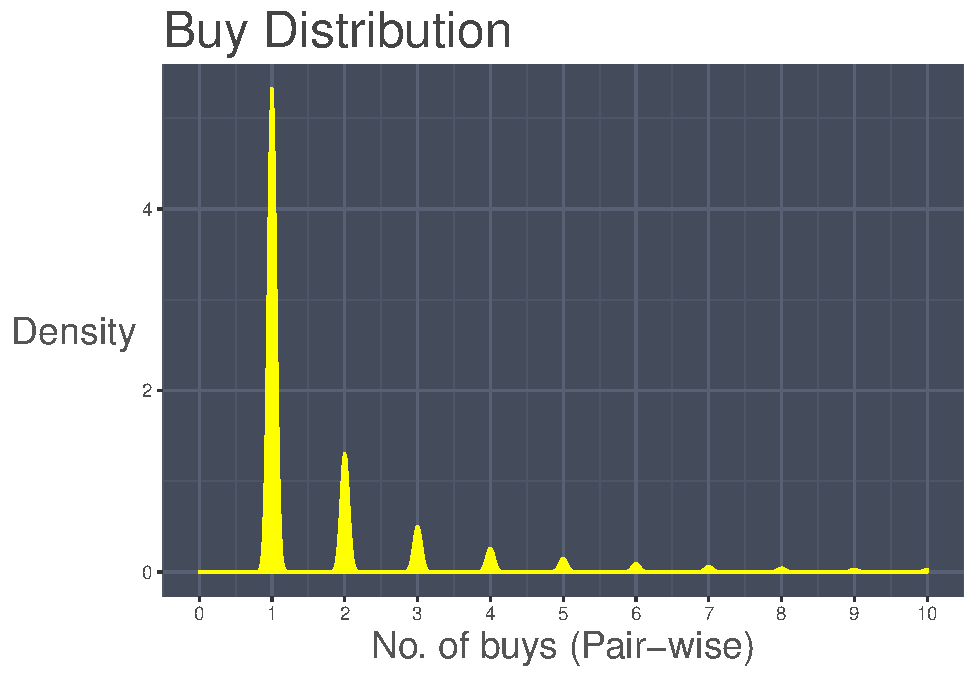
\includegraphics{analysis_files/figure-latex/unnamed-chunk-48-1.pdf}
\#\#\#Similarly, we'll generate the `sell' distribution. This will
contain the frequency of number of sells performed by users

\begin{Shaded}
\begin{Highlighting}[]
\NormalTok{omisego.pair.users.sells <-}\StringTok{ }\NormalTok{filteredOmisegoTX }\OperatorTok\StringTok{ }\KeywordTok{group_by}\NormalTok{(fromAddress) }\OperatorTok\StringTok{ }\KeywordTok{summarise}\NormalTok{(}\DataTypeTok{n =} \KeywordTok{n}\NormalTok{(), }\DataTypeTok{sumAmount=}\KeywordTok{sum}\NormalTok{(tokenAmount))}
\KeywordTok{head}\NormalTok{(omisego.pair.users.sells)}
\end{Highlighting}
\end{Shaded}

\begin{verbatim}
## # A tibble: 6 x 3
##   fromAddress     n sumAmount
##         <int> <int>     <dbl>
## 1           0     1   4.00e19
## 2           2     1   9.00e18
## 3           4   123   1.74e23
## 4           5 48528   3.18e25
## 5           6 10806   3.65e24
## 6           7   139   2.78e24
\end{verbatim}

\subsubsection{\texorpdfstring{Plotting density distribution for `Sell'
transactions}{Plotting density distribution for Sell transactions}}\label{plotting-density-distribution-for-sell-transactions-2}

\begin{Shaded}
\begin{Highlighting}[]
\KeywordTok{ggplot}\NormalTok{(}\DataTypeTok{data=}\NormalTok{omisego.pair.users.sells, }\KeywordTok{aes}\NormalTok{(omisego.pair.users.sells}\OperatorTok{$}\NormalTok{n)) }\OperatorTok{+}\StringTok{ }
\StringTok{  }\KeywordTok{geom_density}\NormalTok{(}\DataTypeTok{fill=}\StringTok{'cyan'}\NormalTok{, }\DataTypeTok{color=}\StringTok{'cyan'}\NormalTok{) }\OperatorTok{+}\StringTok{ }
\StringTok{  }\KeywordTok{scale_x_continuous}\NormalTok{(}\DataTypeTok{breaks=}\KeywordTok{seq}\NormalTok{(}\DecValTok{0}\NormalTok{,}\DecValTok{10}\NormalTok{,}\DecValTok{1}\NormalTok{), }\DataTypeTok{limits=}\KeywordTok{c}\NormalTok{(}\DecValTok{0}\NormalTok{,}\DecValTok{10}\NormalTok{)) }\OperatorTok{+}\StringTok{ }
\StringTok{  }\KeywordTok{xlab}\NormalTok{(}\StringTok{"No. of sells (Pair-wise)"}\NormalTok{) }\OperatorTok{+}
\StringTok{  }\KeywordTok{ylab}\NormalTok{(}\StringTok{"Density"}\NormalTok{) }\OperatorTok{+}\StringTok{ }
\StringTok{  }\KeywordTok{ggtitle}\NormalTok{(}\StringTok{"Sell Distribution"}\NormalTok{) }\OperatorTok{+}\StringTok{ }
\StringTok{  }\KeywordTok{theme}\NormalTok{(}\DataTypeTok{text =} \KeywordTok{element_text}\NormalTok{(}\DataTypeTok{color =} \StringTok{"#444444"}\NormalTok{)}
\NormalTok{        ,}\DataTypeTok{panel.background =} \KeywordTok{element_rect}\NormalTok{(}\DataTypeTok{fill =} \StringTok{'#444B5A'}\NormalTok{)}
\NormalTok{        ,}\DataTypeTok{panel.grid.minor =} \KeywordTok{element_line}\NormalTok{(}\DataTypeTok{color =} \StringTok{'#4d5566'}\NormalTok{)}
\NormalTok{        ,}\DataTypeTok{panel.grid.major =} \KeywordTok{element_line}\NormalTok{(}\DataTypeTok{color =} \StringTok{'#586174'}\NormalTok{)}
\NormalTok{        ,}\DataTypeTok{plot.title =} \KeywordTok{element_text}\NormalTok{(}\DataTypeTok{size =} \DecValTok{24}\NormalTok{)}
\NormalTok{        ,}\DataTypeTok{axis.title =} \KeywordTok{element_text}\NormalTok{(}\DataTypeTok{size =} \DecValTok{18}\NormalTok{, }\DataTypeTok{color =} \StringTok{'#555555'}\NormalTok{)}
\NormalTok{        ,}\DataTypeTok{axis.title.y =} \KeywordTok{element_text}\NormalTok{(}\DataTypeTok{vjust =}\NormalTok{ .}\DecValTok{5}\NormalTok{, }\DataTypeTok{angle =} \DecValTok{0}\NormalTok{)}
\NormalTok{        ,}\DataTypeTok{axis.title.x =} \KeywordTok{element_text}\NormalTok{(}\DataTypeTok{hjust =}\NormalTok{ .}\DecValTok{5}\NormalTok{)}
\NormalTok{  ) }
\end{Highlighting}
\end{Shaded}

\begin{verbatim}
## Warning: Removed 3321 rows containing non-finite values (stat_density).
\end{verbatim}

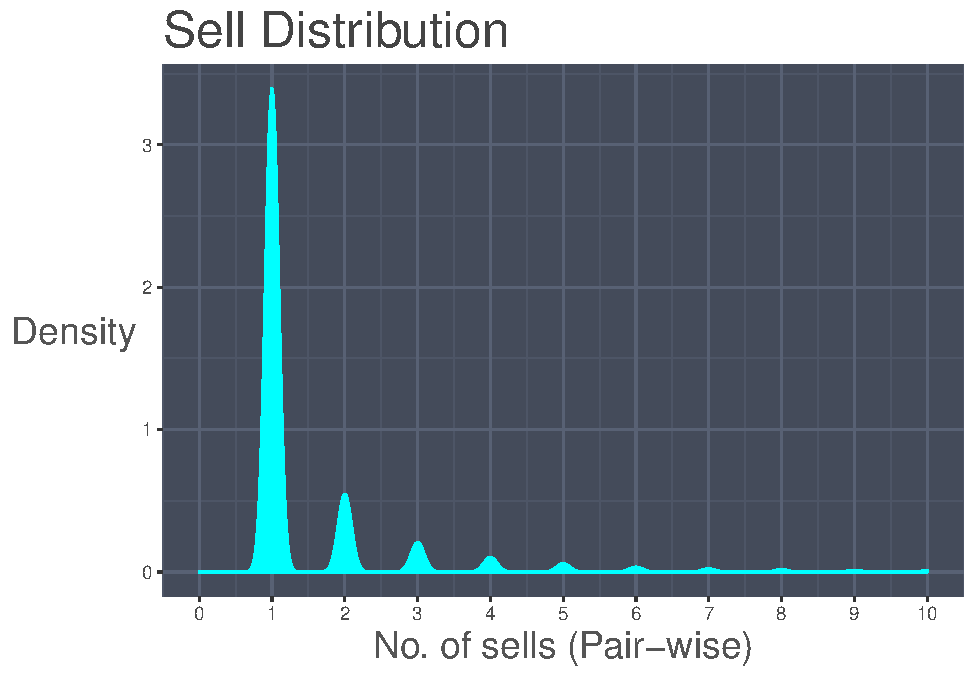
\includegraphics{analysis_files/figure-latex/unnamed-chunk-50-1.pdf}
\#\#\#Now that we have seen density distributions for both types of
transactions, we'll individually fit the data in different distribution
models

\begin{Shaded}
\begin{Highlighting}[]
\NormalTok{omisego.fit.buy.norm <-}\StringTok{ }\KeywordTok{fitdist}\NormalTok{(omisego.pair.users.buys}\OperatorTok{$}\NormalTok{n, }\StringTok{"norm"}\NormalTok{)}
\NormalTok{omisego.fit.buy.weibull <-}\StringTok{ }\KeywordTok{fitdist}\NormalTok{(omisego.pair.users.buys}\OperatorTok{$}\NormalTok{n, }\StringTok{"weibull"}\NormalTok{)}
\NormalTok{omisego.fit.buy.gamma <-}\StringTok{ }\KeywordTok{fitdist}\NormalTok{(omisego.pair.users.buys}\OperatorTok{$}\NormalTok{n, }\StringTok{"gamma"}\NormalTok{)}
\NormalTok{omisego.fit.buy.lnorm <-}\StringTok{ }\KeywordTok{fitdist}\NormalTok{(omisego.pair.users.buys}\OperatorTok{$}\NormalTok{n, }\StringTok{"lnorm"}\NormalTok{)}
\NormalTok{omisego.fit.buy.exp <-}\StringTok{ }\KeywordTok{fitdist}\NormalTok{(omisego.pair.users.buys}\OperatorTok{$}\NormalTok{n, }\StringTok{"exp"}\NormalTok{)}
\NormalTok{omisego.fit.buy.logis <-}\StringTok{ }\KeywordTok{fitdist}\NormalTok{(omisego.pair.users.buys}\OperatorTok{$}\NormalTok{n, }\StringTok{"logis"}\NormalTok{)}
\end{Highlighting}
\end{Shaded}

\subsubsection{\texorpdfstring{Plotting all distributions and check
which one satisfies our `Buy'
distribution}{Plotting all distributions and check which one satisfies our Buy distribution}}\label{plotting-all-distributions-and-check-which-one-satisfies-our-buy-distribution-2}

\begin{Shaded}
\begin{Highlighting}[]
\NormalTok{plot.legend <-}\StringTok{ }\KeywordTok{c}\NormalTok{(}\StringTok{"Normal"}\NormalTok{, }\StringTok{"Weibull"}\NormalTok{, }\StringTok{"lognormal"}\NormalTok{, }\StringTok{"gamma"}\NormalTok{, }\StringTok{"exponential"}\NormalTok{, }\StringTok{"logistic"}\NormalTok{)}
\KeywordTok{denscomp}\NormalTok{(}\KeywordTok{list}\NormalTok{(omisego.fit.buy.norm,omisego.fit.buy.weibull , omisego.fit.buy.lnorm, omisego.fit.buy.gamma, omisego.fit.buy.exp,omisego.fit.buy.logis), }\DataTypeTok{legendtext =}\NormalTok{ plot.legend, }\DataTypeTok{xlim=}\KeywordTok{c}\NormalTok{(}\DecValTok{0}\NormalTok{,}\DecValTok{10}\NormalTok{), }\DataTypeTok{ylim=}\KeywordTok{c}\NormalTok{(}\DecValTok{0}\NormalTok{,}\FloatTok{0.7}\NormalTok{))}
\end{Highlighting}
\end{Shaded}

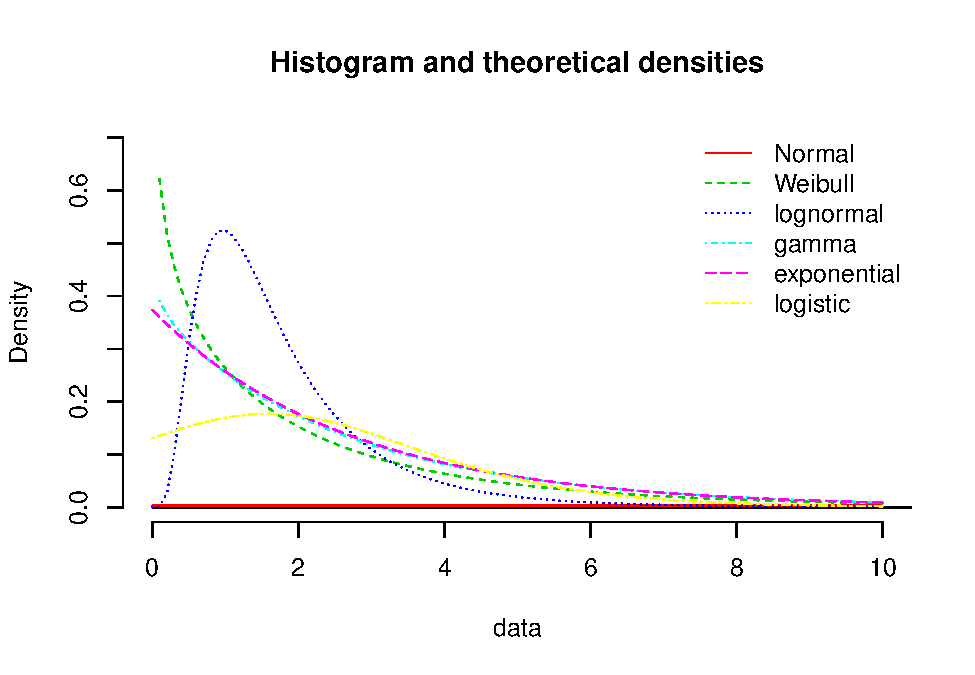
\includegraphics{analysis_files/figure-latex/unnamed-chunk-52-1.pdf}

\begin{Shaded}
\begin{Highlighting}[]
\KeywordTok{gofstat}\NormalTok{(}\KeywordTok{list}\NormalTok{(omisego.fit.buy.norm,omisego.fit.buy.weibull , omisego.fit.buy.lnorm, omisego.fit.buy.gamma, omisego.fit.buy.exp,omisego.fit.buy.logis),}\DataTypeTok{fitnames =} \KeywordTok{c}\NormalTok{(}\StringTok{"Normal"}\NormalTok{, }\StringTok{"Weibull"}\NormalTok{, }\StringTok{"Lognormal"}\NormalTok{, }\StringTok{"Gamma"}\NormalTok{, }\StringTok{"Exponential"}\NormalTok{, }\StringTok{"Logistic"}\NormalTok{))}
\end{Highlighting}
\end{Shaded}

\begin{verbatim}
## Goodness-of-fit statistics
##                                    Normal      Weibull    Lognormal
## Kolmogorov-Smirnov statistic 4.952826e-01 4.225091e-01 3.897757e-01
## Cramer-von Mises statistic   3.391556e+04 1.456020e+04 1.181344e+04
## Anderson-Darling statistic            Inf          Inf          Inf
##                                     Gamma  Exponential     Logistic
## Kolmogorov-Smirnov statistic 3.478873e-01 3.581465e-01 3.964921e-01
## Cramer-von Mises statistic   1.545214e+04 1.575061e+04 1.459751e+04
## Anderson-Darling statistic            Inf          Inf          Inf
## 
## Goodness-of-fit criteria
##                                 Normal Weibull Lognormal   Gamma
## Akaike's Information Criterion 5339492 1548641   1131323 1661562
## Bayesian Information Criterion 5339514 1548663   1131345 1661584
##                                Exponential Logistic
## Akaike's Information Criterion     1662229  2171728
## Bayesian Information Criterion     1662240  2171750
\end{verbatim}

\paragraph{From the goodness of fit statistics and the previous graph,
it seems lognormal is a better fit than the
rest.}\label{from-the-goodness-of-fit-statistics-and-the-previous-graph-it-seems-lognormal-is-a-better-fit-than-the-rest.-2}

\paragraph{Estimating parmaters for this
distribution}\label{estimating-parmaters-for-this-distribution-4}

\begin{Shaded}
\begin{Highlighting}[]
\NormalTok{omisego.fit.buy.lnorm}
\end{Highlighting}
\end{Shaded}

\begin{verbatim}
## Fitting of the distribution ' lnorm ' by maximum likelihood 
## Parameters:
##          estimate   Std. Error
## meanlog 0.3736658 0.0009923673
## sdlog   0.6423653 0.0007017020
\end{verbatim}

\begin{Shaded}
\begin{Highlighting}[]
\NormalTok{omisego.ests.buys <-}\StringTok{ }\KeywordTok{bootdist}\NormalTok{(omisego.fit.buy.lnorm, }\DataTypeTok{niter =} \DecValTok{100}\NormalTok{)}
\KeywordTok{summary}\NormalTok{(omisego.ests.buys)}
\end{Highlighting}
\end{Shaded}

\begin{verbatim}
## Parametric bootstrap medians and 95% percentile CI 
##            Median      2.5%     97.5%
## meanlog 0.3738366 0.3718815 0.3756118
## sdlog   0.6423317 0.6409362 0.6436749
\end{verbatim}

\paragraph{Now fitting distributions for sell
transactions.}\label{now-fitting-distributions-for-sell-transactions.-1}

\begin{Shaded}
\begin{Highlighting}[]
\NormalTok{omisego.fit.sell.norm <-}\StringTok{ }\KeywordTok{fitdist}\NormalTok{(omisego.pair.users.sells}\OperatorTok{$}\NormalTok{n, }\StringTok{"norm"}\NormalTok{)}
\NormalTok{omisego.fit.sell.weibull <-}\StringTok{ }\KeywordTok{fitdist}\NormalTok{(omisego.pair.users.sells}\OperatorTok{$}\NormalTok{n, }\StringTok{"weibull"}\NormalTok{)}
\NormalTok{omisego.fit.sell.gamma <-}\StringTok{ }\KeywordTok{fitdist}\NormalTok{(omisego.pair.users.sells}\OperatorTok{$}\NormalTok{n, }\StringTok{"gamma"}\NormalTok{)}
\NormalTok{omisego.fit.sell.lnorm <-}\StringTok{ }\KeywordTok{fitdist}\NormalTok{(omisego.pair.users.sells}\OperatorTok{$}\NormalTok{n, }\StringTok{"lnorm"}\NormalTok{)}
\NormalTok{omisego.fit.sell.exp <-}\StringTok{ }\KeywordTok{fitdist}\NormalTok{(omisego.pair.users.sells}\OperatorTok{$}\NormalTok{n, }\StringTok{"exp"}\NormalTok{)}
\NormalTok{omisego.fit.sell.logis <-}\StringTok{ }\KeywordTok{fitdist}\NormalTok{(omisego.pair.users.sells}\OperatorTok{$}\NormalTok{n, }\StringTok{"logis"}\NormalTok{)}
\end{Highlighting}
\end{Shaded}

\paragraph{\texorpdfstring{Plotting all distributions and check which
one satisfies our `Sell'
distribution}{Plotting all distributions and check which one satisfies our Sell distribution}}\label{plotting-all-distributions-and-check-which-one-satisfies-our-sell-distribution-2}

\begin{Shaded}
\begin{Highlighting}[]
\NormalTok{plot.legend <-}\StringTok{ }\KeywordTok{c}\NormalTok{(}\StringTok{"Normal"}\NormalTok{,}\StringTok{"Weibull"}\NormalTok{, }\StringTok{"lognormal"}\NormalTok{, }\StringTok{"gamma"}\NormalTok{, }\StringTok{"exponential"}\NormalTok{, }\StringTok{"logistic"}\NormalTok{)}
\KeywordTok{denscomp}\NormalTok{(}\KeywordTok{list}\NormalTok{(omisego.fit.sell.norm, omisego.fit.sell.weibull, omisego.fit.sell.lnorm, omisego.fit.sell.gamma, omisego.fit.sell.exp,omisego.fit.sell.logis), }\DataTypeTok{legendtext =}\NormalTok{ plot.legend, }\DataTypeTok{xlim=}\KeywordTok{c}\NormalTok{(}\DecValTok{0}\NormalTok{,}\DecValTok{10}\NormalTok{), }\DataTypeTok{ylim=}\KeywordTok{c}\NormalTok{(}\DecValTok{0}\NormalTok{,}\DecValTok{1}\NormalTok{))}
\end{Highlighting}
\end{Shaded}

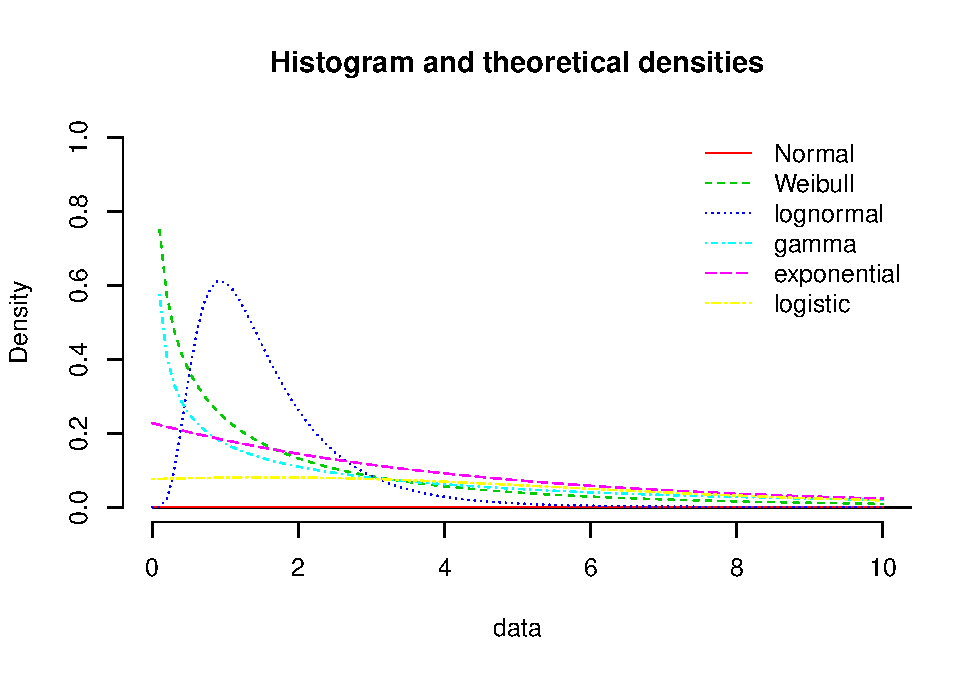
\includegraphics{analysis_files/figure-latex/unnamed-chunk-57-1.pdf}

\begin{Shaded}
\begin{Highlighting}[]
\KeywordTok{gofstat}\NormalTok{(}\KeywordTok{list}\NormalTok{(omisego.fit.sell.norm, omisego.fit.sell.weibull, omisego.fit.sell.lnorm, omisego.fit.sell.gamma, omisego.fit.sell.exp,omisego.fit.sell.logis),}\DataTypeTok{fitnames =} \KeywordTok{c}\NormalTok{(}\StringTok{"Normal"}\NormalTok{, }\StringTok{"Weibull"}\NormalTok{, }\StringTok{"Lognormal"}\NormalTok{, }\StringTok{"Gamma"}\NormalTok{, }\StringTok{"Exponential"}\NormalTok{, }\StringTok{"Logistic"}\NormalTok{))}
\end{Highlighting}
\end{Shaded}

\begin{verbatim}
## Goodness-of-fit statistics
##                                    Normal      Weibull    Lognormal
## Kolmogorov-Smirnov statistic 4.969855e-01     0.459155 4.387477e-01
## Cramer-von Mises statistic   2.110318e+04 12148.141554 1.018560e+04
## Anderson-Darling statistic            Inf          Inf          Inf
##                                     Gamma  Exponential     Logistic
## Kolmogorov-Smirnov statistic 4.041902e-01 5.564261e-01 4.578377e-01
## Cramer-von Mises statistic   1.499422e+04 2.505084e+04 1.465832e+04
## Anderson-Darling statistic            Inf          Inf          Inf
## 
## Goodness-of-fit criteria
##                                 Normal  Weibull Lognormal   Gamma
## Akaike's Information Criterion 3843712 941355.8  593245.4 1171795
## Bayesian Information Criterion 3843733 941376.7  593266.3 1171816
##                                Exponential Logistic
## Akaike's Information Criterion     1266150  1773038
## Bayesian Information Criterion     1266160  1773059
\end{verbatim}

\paragraph{From the goodness of fit statistics and the previous graph,
it seems lognormal is a better fit than the
rest}\label{from-the-goodness-of-fit-statistics-and-the-previous-graph-it-seems-lognormal-is-a-better-fit-than-the-rest-2}

\paragraph{Estimating parmaters for this
distribution}\label{estimating-parmaters-for-this-distribution-5}

\begin{Shaded}
\begin{Highlighting}[]
\NormalTok{omisego.fit.sell.lnorm}
\end{Highlighting}
\end{Shaded}

\begin{verbatim}
## Fitting of the distribution ' lnorm ' by maximum likelihood 
## Parameters:
##          estimate   Std. Error
## meanlog 0.2726650 0.0011642454
## sdlog   0.5884083 0.0008232351
\end{verbatim}

\begin{Shaded}
\begin{Highlighting}[]
\NormalTok{omisego.ests.sells <-}\StringTok{ }\KeywordTok{bootdist}\NormalTok{(omisego.fit.sell.lnorm, }\DataTypeTok{niter =} \DecValTok{100}\NormalTok{)}
\KeywordTok{summary}\NormalTok{(omisego.ests.sells)}
\end{Highlighting}
\end{Shaded}

\begin{verbatim}
## Parametric bootstrap medians and 95% percentile CI 
##            Median      2.5%     97.5%
## meanlog 0.2730199 0.2706834 0.2748500
## sdlog   0.5883249 0.5867979 0.5898678
\end{verbatim}

\section{Question 2}\label{question-2}

\subsubsection{To get top buyers and sellers in the 3 tokens, we'll
arrange the data in descending order for each of the summarised
data}\label{to-get-top-buyers-and-sellers-in-the-3-tokens-well-arrange-the-data-in-descending-order-for-each-of-the-summarised-data}

\begin{Shaded}
\begin{Highlighting}[]
\NormalTok{golem.buyers <-}\StringTok{ }\NormalTok{pair.users.buys }\OperatorTok\StringTok{ }\KeywordTok{arrange}\NormalTok{(}\OperatorTok{-}\NormalTok{n)}
\NormalTok{golem.sellers <-}\StringTok{ }\NormalTok{pair.users.sells }\OperatorTok\StringTok{ }\KeywordTok{arrange}\NormalTok{(}\OperatorTok{-}\NormalTok{n)}

\NormalTok{yocoin.buyers <-}\StringTok{ }\NormalTok{yocoin.pair.users.buys }\OperatorTok\StringTok{ }\KeywordTok{arrange}\NormalTok{(}\OperatorTok{-}\NormalTok{n)}
\NormalTok{yocoin.sellers <-}\StringTok{ }\NormalTok{yocoin.pair.users.sells }\OperatorTok\StringTok{ }\KeywordTok{arrange}\NormalTok{(}\OperatorTok{-}\NormalTok{n)}

\NormalTok{omisego.buyers <-}\StringTok{ }\NormalTok{omisego.pair.users.buys }\OperatorTok\StringTok{ }\KeywordTok{arrange}\NormalTok{(}\OperatorTok{-}\NormalTok{n)}
\NormalTok{omisego.sellers <-}\StringTok{ }\NormalTok{omisego.pair.users.sells }\OperatorTok\StringTok{ }\KeywordTok{arrange}\NormalTok{(}\OperatorTok{-}\NormalTok{n)}
\end{Highlighting}
\end{Shaded}

\subsection{\texorpdfstring{We'll create a regression model for token
`Golem'}{We'll create a regression model for token Golem}}\label{well-create-a-regression-model-for-token-golem}

\subsubsection{Taking K-value as 20 i.e.~top 20 buyers, we'll build a
regression model based on number of buys with total tokenAmount as
outcome}\label{taking-k-value-as-20-i.e.top-20-buyers-well-build-a-regression-model-based-on-number-of-buys-with-total-tokenamount-as-outcome}

\begin{Shaded}
\begin{Highlighting}[]
\NormalTok{golem.buyers.}\DecValTok{20}\NormalTok{ <-}\StringTok{ }\KeywordTok{head}\NormalTok{(golem.buyers,}\DecValTok{20}\NormalTok{)}
\NormalTok{golem.buyers.}\DecValTok{20}
\end{Highlighting}
\end{Shaded}

\begin{verbatim}
## # A tibble: 20 x 3
##    toAddress     n sumAmount
##        <int> <int>     <dbl>
##  1   2335455 93293   2.86e26
##  2   4067724  7020   4.10e25
##  3   4092385  5452   1.33e26
##  4        49  5192   1.62e26
##  5         5  3709   5.15e25
##  6     75994  3545   1.15e26
##  7   4067686  3447   1.02e26
##  8    297031  3081   1.24e25
##  9   4067819  2963   1.09e26
## 10    104502  2548   6.20e24
## 11   1444018  2006   3.36e23
## 12    104531  1081   2.50e24
## 13   4067739  1029   1.01e24
## 14   4175170   989   5.88e24
## 15    142341   961   5.19e25
## 16   4068179   960   9.94e23
## 17     40044   782   3.09e24
## 18   4250818   765   1.40e25
## 19   4104950   751   1.56e23
## 20   4067789   685   7.32e24
\end{verbatim}

\paragraph{Creating a scatterplot to check the relation between these
addresses and tokenAmount for their buys in'Golem' token. We'll also
transform the tokenAmount to it's square root value for better
visualization}\label{creating-a-scatterplot-to-check-the-relation-between-these-addresses-and-tokenamount-for-their-buys-ingolem-token.-well-also-transform-the-tokenamount-to-its-square-root-value-for-better-visualization}

\begin{Shaded}
\begin{Highlighting}[]
\CommentTok{#golem.buyers.20.data <- filteredGolemTX[filteredGolemTX$toAddress %in% golem.buyers.20, ]}
\CommentTok{#golem.buyers.20.data$toAddress <- as.character(golem.buyers.20.data$toAddress)}
\KeywordTok{ggplot}\NormalTok{(}\KeywordTok{aes}\NormalTok{(}\DataTypeTok{x=}\NormalTok{n,}\DataTypeTok{y=}\NormalTok{sumAmount), }\DataTypeTok{data =}\NormalTok{ golem.buyers.}\DecValTok{20}\NormalTok{) }\OperatorTok{+}\StringTok{ }
\StringTok{  }\KeywordTok{geom_point}\NormalTok{(}\DataTypeTok{fill=}\StringTok{"orange"}\NormalTok{, }\DataTypeTok{color=}\StringTok{'black'}\NormalTok{, }\DataTypeTok{shape=}\DecValTok{21}\NormalTok{) }\OperatorTok{+}
\StringTok{  }\KeywordTok{scale_y_continuous}\NormalTok{(}\DataTypeTok{trans=}\StringTok{'log2'}\NormalTok{) }\OperatorTok{+}
\StringTok{  }\KeywordTok{xlab}\NormalTok{(}\StringTok{"Buy frequency"}\NormalTok{) }\OperatorTok{+}\StringTok{ }
\StringTok{  }\KeywordTok{xlim}\NormalTok{(}\DecValTok{0}\NormalTok{,}\DecValTok{7200}\NormalTok{) }\OperatorTok{+}\StringTok{ }
\StringTok{  }\KeywordTok{theme}\NormalTok{(}\DataTypeTok{axis.text.x =} \KeywordTok{element_text}\NormalTok{(}\DataTypeTok{angle =} \DecValTok{90}\NormalTok{, }\DataTypeTok{hjust =} \DecValTok{1}\NormalTok{)) }\OperatorTok{+}
\StringTok{  }\KeywordTok{geom_line}\NormalTok{()}
\end{Highlighting}
\end{Shaded}

\begin{verbatim}
## Warning: Removed 1 rows containing missing values (geom_point).
\end{verbatim}

\begin{verbatim}
## Warning: Removed 1 rows containing missing values (geom_path).
\end{verbatim}

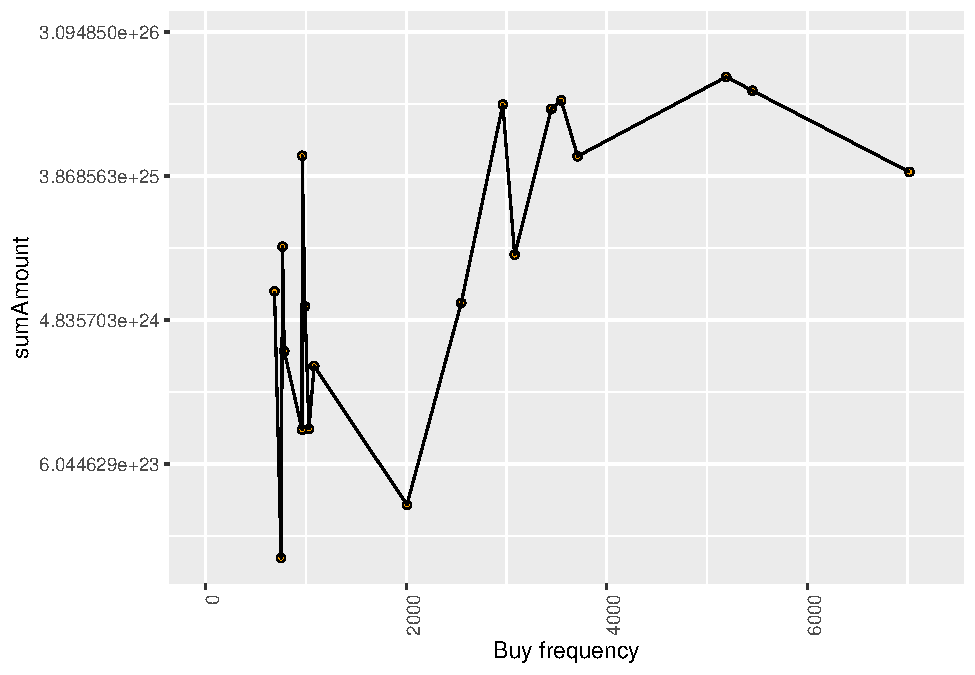
\includegraphics{analysis_files/figure-latex/unnamed-chunk-63-1.pdf}

\begin{Shaded}
\begin{Highlighting}[]
\KeywordTok{cor}\NormalTok{(golem.buyers.}\DecValTok{20}\OperatorTok{$}\NormalTok{n, golem.buyers.}\DecValTok{20}\OperatorTok{$}\NormalTok{sumAmount)}
\end{Highlighting}
\end{Shaded}

\begin{verbatim}
## [1] 0.7613258
\end{verbatim}

\paragraph{We can see that there there some corealtion between the
number of buys and total token
amount}\label{we-can-see-that-there-there-some-corealtion-between-the-number-of-buys-and-total-token-amount}

\begin{Shaded}
\begin{Highlighting}[]
\NormalTok{linearMod <-}\StringTok{ }\KeywordTok{lm}\NormalTok{(sumAmount }\OperatorTok{~}\StringTok{ }\NormalTok{n, }\DataTypeTok{data=}\NormalTok{golem.buyers.}\DecValTok{20}\NormalTok{)  }\CommentTok{# build linear regression model on full data}
\KeywordTok{print}\NormalTok{(linearMod)}
\end{Highlighting}
\end{Shaded}

\begin{verbatim}
## 
## Call:
## lm(formula = sumAmount ~ n, data = golem.buyers.20)
## 
## Coefficients:
## (Intercept)            n  
##   3.553e+25    2.810e+21
\end{verbatim}

\begin{Shaded}
\begin{Highlighting}[]
\KeywordTok{summary}\NormalTok{(linearMod) }
\end{Highlighting}
\end{Shaded}

\begin{verbatim}
## 
## Call:
## lm(formula = sumAmount ~ n, data = golem.buyers.20)
## 
## Residuals:
##        Min         1Q     Median         3Q        Max 
## -4.083e+25 -3.618e+25 -2.692e+25  2.438e+25  1.117e+26 
## 
## Coefficients:
##              Estimate Std. Error t value Pr(>|t|)    
## (Intercept) 3.553e+25  1.189e+25   2.988  0.00788 ** 
## n           2.810e+21  5.641e+20   4.982 9.66e-05 ***
## ---
## Signif. codes:  0 '***' 0.001 '**' 0.01 '*' 0.05 '.' 0.1 ' ' 1
## 
## Residual standard error: 5.014e+25 on 18 degrees of freedom
## Multiple R-squared:  0.5796, Adjusted R-squared:  0.5563 
## F-statistic: 24.82 on 1 and 18 DF,  p-value: 9.658e-05
\end{verbatim}

\begin{Shaded}
\begin{Highlighting}[]
\NormalTok{modelSummary <-}\StringTok{ }\KeywordTok{summary}\NormalTok{(linearMod)  }\CommentTok{# capture model summary as an object}
\NormalTok{modelCoeffs <-}\StringTok{ }\NormalTok{modelSummary}\OperatorTok{$}\NormalTok{coefficients  }\CommentTok{# model coefficients}
\NormalTok{beta.estimate <-}\StringTok{ }\NormalTok{modelCoeffs[}\StringTok{"n"}\NormalTok{, }\StringTok{"Estimate"}\NormalTok{]  }\CommentTok{# get beta estimate for frequency of buys}
\NormalTok{std.error <-}\StringTok{ }\NormalTok{modelCoeffs[}\StringTok{"n"}\NormalTok{, }\StringTok{"Std. Error"}\NormalTok{]  }\CommentTok{# get std.error for frequency of buys}
\NormalTok{t_value <-}\StringTok{ }\NormalTok{beta.estimate}\OperatorTok{/}\NormalTok{std.error  }\CommentTok{# calc t statistic}
\NormalTok{p_value <-}\StringTok{ }\DecValTok{2}\OperatorTok{*}\KeywordTok{pt}\NormalTok{(}\OperatorTok{-}\KeywordTok{abs}\NormalTok{(t_value), }\DataTypeTok{df=}\KeywordTok{nrow}\NormalTok{(golem.buyers.}\DecValTok{20}\NormalTok{)}\OperatorTok{-}\KeywordTok{ncol}\NormalTok{(golem.buyers.}\DecValTok{20}\NormalTok{))  }\CommentTok{# calc p Value}
\NormalTok{f_statistic <-}\StringTok{ }\NormalTok{linearMod}\OperatorTok{$}\NormalTok{fstatistic[}\DecValTok{1}\NormalTok{]  }\CommentTok{# fstatistic}
\NormalTok{f <-}\StringTok{ }\KeywordTok{summary}\NormalTok{(linearMod)}\OperatorTok{$}\NormalTok{fstatistic  }\CommentTok{# parameters for model p-value calc}
\NormalTok{model_p <-}\StringTok{ }\KeywordTok{pf}\NormalTok{(f[}\DecValTok{1}\NormalTok{], f[}\DecValTok{2}\NormalTok{], f[}\DecValTok{3}\NormalTok{], }\DataTypeTok{lower=}\OtherTok{FALSE}\NormalTok{)}
\end{Highlighting}
\end{Shaded}

\begin{Shaded}
\begin{Highlighting}[]
\NormalTok{p_value}
\end{Highlighting}
\end{Shaded}

\begin{verbatim}
## [1] 0.0001138393
\end{verbatim}

\paragraph{Akaike's information criterion - AIC (Akaike, 1974); We'll
use this criteria to determine the best linear model. Lower score is
preferred.}\label{akaikes-information-criterion---aic-akaike-1974-well-use-this-criteria-to-determine-the-best-linear-model.-lower-score-is-preferred.}

\begin{Shaded}
\begin{Highlighting}[]
\KeywordTok{AIC}\NormalTok{(linearMod)}
\end{Highlighting}
\end{Shaded}

\begin{verbatim}
## [1] 2427.724
\end{verbatim}

\subsubsection{Taking K-value as 100 i.e.~top 100 buyers, we'll build a
regression model based on number of buys with total tokenAmount as
outcome}\label{taking-k-value-as-100-i.e.top-100-buyers-well-build-a-regression-model-based-on-number-of-buys-with-total-tokenamount-as-outcome}

\begin{Shaded}
\begin{Highlighting}[]
\NormalTok{golem.buyers.}\DecValTok{100}\NormalTok{ <-}\StringTok{ }\KeywordTok{head}\NormalTok{(golem.buyers,}\DecValTok{100}\NormalTok{)}
\NormalTok{golem.buyers.}\DecValTok{100}
\end{Highlighting}
\end{Shaded}

\begin{verbatim}
## # A tibble: 100 x 3
##    toAddress     n sumAmount
##        <int> <int>     <dbl>
##  1   2335455 93293   2.86e26
##  2   4067724  7020   4.10e25
##  3   4092385  5452   1.33e26
##  4        49  5192   1.62e26
##  5         5  3709   5.15e25
##  6     75994  3545   1.15e26
##  7   4067686  3447   1.02e26
##  8    297031  3081   1.24e25
##  9   4067819  2963   1.09e26
## 10    104502  2548   6.20e24
## # ... with 90 more rows
\end{verbatim}

\begin{Shaded}
\begin{Highlighting}[]
\KeywordTok{cor}\NormalTok{(golem.buyers.}\DecValTok{100}\OperatorTok{$}\NormalTok{n, golem.buyers.}\DecValTok{100}\OperatorTok{$}\NormalTok{sumAmount)}
\end{Highlighting}
\end{Shaded}

\begin{verbatim}
## [1] 0.7634644
\end{verbatim}

\begin{Shaded}
\begin{Highlighting}[]
\NormalTok{linearMod2 <-}\StringTok{ }\KeywordTok{lm}\NormalTok{(sumAmount }\OperatorTok{~}\StringTok{ }\NormalTok{n, }\DataTypeTok{data=}\NormalTok{golem.buyers.}\DecValTok{100}\NormalTok{)  }\CommentTok{# build linear regression model on full data}
\KeywordTok{print}\NormalTok{(linearMod)}
\end{Highlighting}
\end{Shaded}

\begin{verbatim}
## 
## Call:
## lm(formula = sumAmount ~ n, data = golem.buyers.20)
## 
## Coefficients:
## (Intercept)            n  
##   3.553e+25    2.810e+21
\end{verbatim}

\begin{Shaded}
\begin{Highlighting}[]
\NormalTok{modelSummary2 <-}\StringTok{ }\KeywordTok{summary}\NormalTok{(linearMod2)  }\CommentTok{# capture model summary as an object}
\NormalTok{modelCoeffs2 <-}\StringTok{ }\NormalTok{modelSummary2}\OperatorTok{$}\NormalTok{coefficients  }\CommentTok{# model coefficients}
\NormalTok{beta.estimate2 <-}\StringTok{ }\NormalTok{modelCoeffs2[}\StringTok{"n"}\NormalTok{, }\StringTok{"Estimate"}\NormalTok{]  }\CommentTok{# get beta estimate for frequency of buys}
\NormalTok{std.error2 <-}\StringTok{ }\NormalTok{modelCoeffs2[}\StringTok{"n"}\NormalTok{, }\StringTok{"Std. Error"}\NormalTok{]  }\CommentTok{# get std.error for frequency of buys}
\NormalTok{t_value2 <-}\StringTok{ }\NormalTok{beta.estimate2}\OperatorTok{/}\NormalTok{std.error2  }\CommentTok{# calc t statistic}
\NormalTok{p_value2 <-}\StringTok{ }\DecValTok{2}\OperatorTok{*}\KeywordTok{pt}\NormalTok{(}\OperatorTok{-}\KeywordTok{abs}\NormalTok{(t_value2), }\DataTypeTok{df=}\KeywordTok{nrow}\NormalTok{(golem.buyers.}\DecValTok{100}\NormalTok{)}\OperatorTok{-}\KeywordTok{ncol}\NormalTok{(golem.buyers.}\DecValTok{100}\NormalTok{))  }\CommentTok{# calc p Value}
\NormalTok{f_statistic2 <-}\StringTok{ }\NormalTok{linearMod}\OperatorTok{$}\NormalTok{fstatistic[}\DecValTok{1}\NormalTok{]  }\CommentTok{# fstatistic}
\NormalTok{f2 <-}\StringTok{ }\KeywordTok{summary}\NormalTok{(linearMod)}\OperatorTok{$}\NormalTok{fstatistic  }\CommentTok{# parameters for model p-value calc}
\NormalTok{model_p2 <-}\StringTok{ }\KeywordTok{pf}\NormalTok{(f2[}\DecValTok{1}\NormalTok{], f2[}\DecValTok{2}\NormalTok{], f2[}\DecValTok{3}\NormalTok{], }\DataTypeTok{lower=}\OtherTok{FALSE}\NormalTok{)}
\end{Highlighting}
\end{Shaded}

\begin{Shaded}
\begin{Highlighting}[]
\NormalTok{p_value}
\end{Highlighting}
\end{Shaded}

\begin{verbatim}
## [1] 0.0001138393
\end{verbatim}

\begin{Shaded}
\begin{Highlighting}[]
\KeywordTok{AIC}\NormalTok{(linearMod2)}
\end{Highlighting}
\end{Shaded}

\begin{verbatim}
## [1] 11988.78
\end{verbatim}

\paragraph{For Golem token, the number of buys with K value 20 fares
better than K value of 100; therefore, K-value of 20 is preferred for
number of buys vs totalTokenAmount linear regression
model}\label{for-golem-token-the-number-of-buys-with-k-value-20-fares-better-than-k-value-of-100-therefore-k-value-of-20-is-preferred-for-number-of-buys-vs-totaltokenamount-linear-regression-model}

\subsection{\texorpdfstring{Regression model for token
`Yocoin'}{Regression model for token Yocoin}}\label{regression-model-for-token-yocoin}

\paragraph{Taking K-value as 50 i.e.~top 50 buyers, we'll build a
regression model based on number of buys with total tokenAmount as
outcome}\label{taking-k-value-as-50-i.e.top-50-buyers-well-build-a-regression-model-based-on-number-of-buys-with-total-tokenamount-as-outcome}

\begin{Shaded}
\begin{Highlighting}[]
\NormalTok{yocoin.buyers.}\DecValTok{50}\NormalTok{ <-}\StringTok{ }\KeywordTok{head}\NormalTok{(yocoin.buyers,}\DecValTok{50}\NormalTok{)}
\NormalTok{yocoin.buyers.}\DecValTok{50}
\end{Highlighting}
\end{Shaded}

\begin{verbatim}
## # A tibble: 50 x 3
##    toAddress     n sumAmount
##        <int> <int>     <dbl>
##  1   9911653 14758   2.70e25
##  2    309659  7000   2.22e24
##  3   9912976  6219   2.28e22
##  4   9916042  6110   4.37e21
##  5   9915788  5622   4.71e21
##  6   9913800  4518   9.09e21
##  7   9916338  4286   9.89e20
##  8   9911955  3028   5.17e21
##  9   9912979  3012   1.10e22
## 10   9913169  2879   4.25e21
## # ... with 40 more rows
\end{verbatim}

\paragraph{\texorpdfstring{Creating a scatterplot to check the relation
between the frequency of buys and total tokenAmount in `Yocoin' token.
We'll also transform the tokenAmount to it's square root value for
better
visualization}{Creating a scatterplot to check the relation between the frequency of buys and total tokenAmount in Yocoin token. We'll also transform the tokenAmount to it's square root value for better visualization}}\label{creating-a-scatterplot-to-check-the-relation-between-the-frequency-of-buys-and-total-tokenamount-in-yocoin-token.-well-also-transform-the-tokenamount-to-its-square-root-value-for-better-visualization}

\begin{Shaded}
\begin{Highlighting}[]
\KeywordTok{ggplot}\NormalTok{(}\KeywordTok{aes}\NormalTok{(}\DataTypeTok{x=}\NormalTok{n,}\DataTypeTok{y=}\NormalTok{sumAmount), }\DataTypeTok{data =}\NormalTok{ yocoin.buyers.}\DecValTok{50}\NormalTok{) }\OperatorTok{+}\StringTok{ }
\StringTok{  }\KeywordTok{geom_point}\NormalTok{(}\DataTypeTok{fill=}\StringTok{"orange"}\NormalTok{, }\DataTypeTok{color=}\StringTok{'black'}\NormalTok{, }\DataTypeTok{shape=}\DecValTok{21}\NormalTok{) }\OperatorTok{+}
\StringTok{  }\KeywordTok{scale_y_continuous}\NormalTok{(}\DataTypeTok{trans=}\StringTok{'log2'}\NormalTok{) }\OperatorTok{+}
\StringTok{  }\KeywordTok{xlab}\NormalTok{(}\StringTok{"Buy frequency"}\NormalTok{) }\OperatorTok{+}\StringTok{ }
\StringTok{  }\KeywordTok{xlim}\NormalTok{(}\DecValTok{0}\NormalTok{,}\DecValTok{7200}\NormalTok{) }\OperatorTok{+}\StringTok{ }
\StringTok{  }\KeywordTok{theme}\NormalTok{(}\DataTypeTok{axis.text.x =} \KeywordTok{element_text}\NormalTok{(}\DataTypeTok{angle =} \DecValTok{90}\NormalTok{, }\DataTypeTok{hjust =} \DecValTok{1}\NormalTok{)) }\OperatorTok{+}
\StringTok{  }\KeywordTok{geom_line}\NormalTok{()}
\end{Highlighting}
\end{Shaded}

\begin{verbatim}
## Warning: Removed 1 rows containing missing values (geom_point).
\end{verbatim}

\begin{verbatim}
## Warning: Removed 1 rows containing missing values (geom_path).
\end{verbatim}

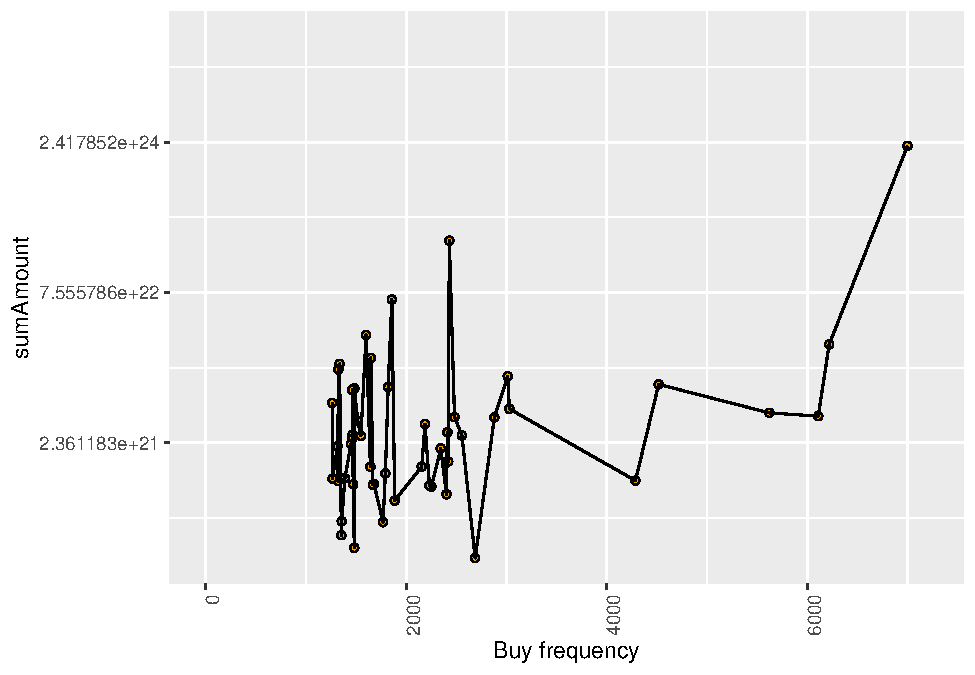
\includegraphics{analysis_files/figure-latex/unnamed-chunk-77-1.pdf}

\begin{Shaded}
\begin{Highlighting}[]
\KeywordTok{cor}\NormalTok{(yocoin.buyers.}\DecValTok{50}\OperatorTok{$}\NormalTok{n, yocoin.buyers.}\DecValTok{50}\OperatorTok{$}\NormalTok{sumAmount)}
\end{Highlighting}
\end{Shaded}

\begin{verbatim}
## [1] 0.811942
\end{verbatim}

\begin{Shaded}
\begin{Highlighting}[]
\NormalTok{linearMod3 <-}\StringTok{ }\KeywordTok{lm}\NormalTok{(sumAmount }\OperatorTok{~}\StringTok{ }\NormalTok{n, }\DataTypeTok{data=}\NormalTok{yocoin.buyers.}\DecValTok{50}\NormalTok{)  }\CommentTok{# build linear regression model on full data}
\KeywordTok{summary}\NormalTok{(linearMod3)}
\end{Highlighting}
\end{Shaded}

\begin{verbatim}
## 
## Call:
## lm(formula = sumAmount ~ n, data = yocoin.buyers.50)
## 
## Residuals:
##        Min         1Q     Median         3Q        Max 
## -5.663e+24 -3.770e+23  5.102e+23  9.562e+23  9.430e+24 
## 
## Coefficients:
##               Estimate Std. Error t value Pr(>|t|)    
## (Intercept) -2.993e+24  4.905e+23  -6.101 1.75e-07 ***
## n            1.396e+21  1.448e+20   9.637 8.39e-13 ***
## ---
## Signif. codes:  0 '***' 0.001 '**' 0.01 '*' 0.05 '.' 0.1 ' ' 1
## 
## Residual standard error: 2.258e+24 on 48 degrees of freedom
## Multiple R-squared:  0.6592, Adjusted R-squared:  0.6522 
## F-statistic: 92.87 on 1 and 48 DF,  p-value: 8.387e-13
\end{verbatim}

\begin{Shaded}
\begin{Highlighting}[]
\NormalTok{modelSummary3 <-}\StringTok{ }\KeywordTok{summary}\NormalTok{(linearMod3)  }\CommentTok{# capture model summary as an object}
\NormalTok{modelCoeffs3 <-}\StringTok{ }\NormalTok{modelSummary3}\OperatorTok{$}\NormalTok{coefficients  }\CommentTok{# model coefficients}
\NormalTok{beta.estimate3 <-}\StringTok{ }\NormalTok{modelCoeffs3[}\StringTok{"n"}\NormalTok{, }\StringTok{"Estimate"}\NormalTok{]  }\CommentTok{# get beta estimate for frequency of buys}
\NormalTok{std.error3 <-}\StringTok{ }\NormalTok{modelCoeffs3[}\StringTok{"n"}\NormalTok{, }\StringTok{"Std. Error"}\NormalTok{]  }\CommentTok{# get std.error for frequency of buys}
\NormalTok{t_value3 <-}\StringTok{ }\NormalTok{beta.estimate3}\OperatorTok{/}\NormalTok{std.error3  }\CommentTok{# calc t statistic}
\NormalTok{p_value3 <-}\StringTok{ }\DecValTok{2}\OperatorTok{*}\KeywordTok{pt}\NormalTok{(}\OperatorTok{-}\KeywordTok{abs}\NormalTok{(t_value3), }\DataTypeTok{df=}\KeywordTok{nrow}\NormalTok{(yocoin.buyers.}\DecValTok{50}\NormalTok{)}\OperatorTok{-}\KeywordTok{ncol}\NormalTok{(yocoin.buyers.}\DecValTok{50}\NormalTok{))  }\CommentTok{# calc p Value}
\NormalTok{f_statistic3 <-}\StringTok{ }\NormalTok{linearMod3}\OperatorTok{$}\NormalTok{fstatistic[}\DecValTok{1}\NormalTok{]  }\CommentTok{# fstatistic}
\NormalTok{f3 <-}\StringTok{ }\KeywordTok{summary}\NormalTok{(linearMod3)}\OperatorTok{$}\NormalTok{fstatistic  }\CommentTok{# parameters for model p-value calc}
\NormalTok{model_p3 <-}\StringTok{ }\KeywordTok{pf}\NormalTok{(f3[}\DecValTok{1}\NormalTok{], f3[}\DecValTok{2}\NormalTok{], f3[}\DecValTok{3}\NormalTok{], }\DataTypeTok{lower=}\OtherTok{FALSE}\NormalTok{)}
\end{Highlighting}
\end{Shaded}

\begin{Shaded}
\begin{Highlighting}[]
\NormalTok{model_p3}
\end{Highlighting}
\end{Shaded}

\begin{verbatim}
##        value 
## 8.387138e-13
\end{verbatim}

\begin{Shaded}
\begin{Highlighting}[]
\KeywordTok{AIC}\NormalTok{(linearMod3)}
\end{Highlighting}
\end{Shaded}

\begin{verbatim}
## [1] 5753.492
\end{verbatim}

\subsubsection{Taking K-value as 200 i.e.~top 200 buyers, we'll build a
regression model based on number of buys with total tokenAmount as
outcome}\label{taking-k-value-as-200-i.e.top-200-buyers-well-build-a-regression-model-based-on-number-of-buys-with-total-tokenamount-as-outcome}

\begin{Shaded}
\begin{Highlighting}[]
\NormalTok{yocoin.buyers.}\DecValTok{200}\NormalTok{ <-}\StringTok{ }\KeywordTok{head}\NormalTok{(yocoin.buyers,}\DecValTok{200}\NormalTok{)}
\NormalTok{yocoin.buyers.}\DecValTok{200}
\end{Highlighting}
\end{Shaded}

\begin{verbatim}
## # A tibble: 200 x 3
##    toAddress     n sumAmount
##        <int> <int>     <dbl>
##  1   9911653 14758   2.70e25
##  2    309659  7000   2.22e24
##  3   9912976  6219   2.28e22
##  4   9916042  6110   4.37e21
##  5   9915788  5622   4.71e21
##  6   9913800  4518   9.09e21
##  7   9916338  4286   9.89e20
##  8   9911955  3028   5.17e21
##  9   9912979  3012   1.10e22
## 10   9913169  2879   4.25e21
## # ... with 190 more rows
\end{verbatim}

\paragraph{\texorpdfstring{Creating a scatterplot to check the relation
between the frequency of buys and total tokenAmount in `Yocoin' token.
We'll also transform the tokenAmount to it's square root value for
better
visualization}{Creating a scatterplot to check the relation between the frequency of buys and total tokenAmount in Yocoin token. We'll also transform the tokenAmount to it's square root value for better visualization}}\label{creating-a-scatterplot-to-check-the-relation-between-the-frequency-of-buys-and-total-tokenamount-in-yocoin-token.-well-also-transform-the-tokenamount-to-its-square-root-value-for-better-visualization-1}

\begin{Shaded}
\begin{Highlighting}[]
\KeywordTok{ggplot}\NormalTok{(}\KeywordTok{aes}\NormalTok{(}\DataTypeTok{x=}\NormalTok{n,}\DataTypeTok{y=}\NormalTok{sumAmount), }\DataTypeTok{data =}\NormalTok{ yocoin.buyers.}\DecValTok{200}\NormalTok{) }\OperatorTok{+}\StringTok{ }
\StringTok{  }\KeywordTok{geom_point}\NormalTok{(}\DataTypeTok{fill=}\StringTok{"orange"}\NormalTok{, }\DataTypeTok{color=}\StringTok{'black'}\NormalTok{, }\DataTypeTok{shape=}\DecValTok{21}\NormalTok{) }\OperatorTok{+}
\StringTok{  }\KeywordTok{scale_y_continuous}\NormalTok{(}\DataTypeTok{trans=}\StringTok{'log2'}\NormalTok{) }\OperatorTok{+}
\StringTok{  }\KeywordTok{xlab}\NormalTok{(}\StringTok{"Buy frequency"}\NormalTok{) }\OperatorTok{+}\StringTok{ }
\StringTok{  }\KeywordTok{xlim}\NormalTok{(}\DecValTok{0}\NormalTok{,}\DecValTok{7200}\NormalTok{) }\OperatorTok{+}\StringTok{ }
\StringTok{  }\KeywordTok{theme}\NormalTok{(}\DataTypeTok{axis.text.x =} \KeywordTok{element_text}\NormalTok{(}\DataTypeTok{angle =} \DecValTok{90}\NormalTok{, }\DataTypeTok{hjust =} \DecValTok{1}\NormalTok{)) }\OperatorTok{+}
\StringTok{  }\KeywordTok{geom_line}\NormalTok{()}
\end{Highlighting}
\end{Shaded}

\begin{verbatim}
## Warning: Removed 1 rows containing missing values (geom_point).
\end{verbatim}

\begin{verbatim}
## Warning: Removed 1 rows containing missing values (geom_path).
\end{verbatim}

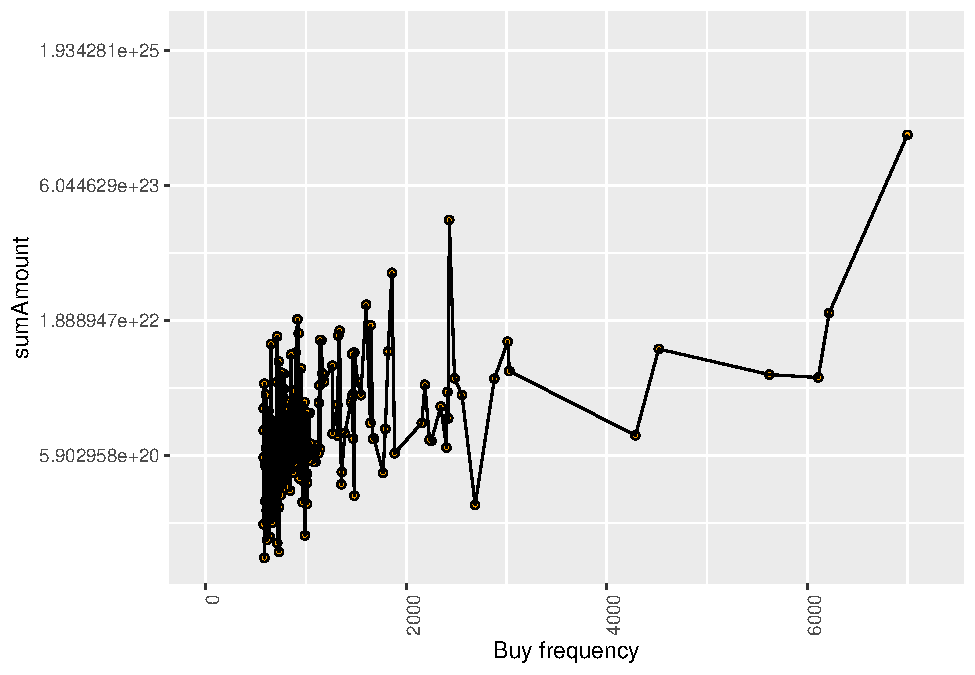
\includegraphics{analysis_files/figure-latex/unnamed-chunk-84-1.pdf}

\begin{Shaded}
\begin{Highlighting}[]
\KeywordTok{cor}\NormalTok{(yocoin.buyers.}\DecValTok{200}\OperatorTok{$}\NormalTok{n, yocoin.buyers.}\DecValTok{200}\OperatorTok{$}\NormalTok{sumAmount)}
\end{Highlighting}
\end{Shaded}

\begin{verbatim}
## [1] 0.7337611
\end{verbatim}

\paragraph{Corelation decrease when we take K-value as 200; taking
k-value as 30, i.e.~top 30
buyers}\label{corelation-decrease-when-we-take-k-value-as-200-taking-k-value-as-30-i.e.top-30-buyers}

\begin{Shaded}
\begin{Highlighting}[]
\NormalTok{yocoin.buyers.}\DecValTok{30}\NormalTok{ <-}\StringTok{ }\KeywordTok{head}\NormalTok{(yocoin.buyers,}\DecValTok{30}\NormalTok{)}
\NormalTok{yocoin.buyers.}\DecValTok{30}
\end{Highlighting}
\end{Shaded}

\begin{verbatim}
## # A tibble: 30 x 3
##    toAddress     n sumAmount
##        <int> <int>     <dbl>
##  1   9911653 14758   2.70e25
##  2    309659  7000   2.22e24
##  3   9912976  6219   2.28e22
##  4   9916042  6110   4.37e21
##  5   9915788  5622   4.71e21
##  6   9913800  4518   9.09e21
##  7   9916338  4286   9.89e20
##  8   9911955  3028   5.17e21
##  9   9912979  3012   1.10e22
## 10   9913169  2879   4.25e21
## # ... with 20 more rows
\end{verbatim}

\begin{Shaded}
\begin{Highlighting}[]
\KeywordTok{cor}\NormalTok{(yocoin.buyers.}\DecValTok{30}\OperatorTok{$}\NormalTok{n, yocoin.buyers.}\DecValTok{30}\OperatorTok{$}\NormalTok{sumAmount)}
\end{Highlighting}
\end{Shaded}

\begin{verbatim}
## [1] 0.844551
\end{verbatim}

\paragraph{We observe that corelation increases when we take a lesser
k-value. We'll proceed with this value and create the regression
model}\label{we-observe-that-corelation-increases-when-we-take-a-lesser-k-value.-well-proceed-with-this-value-and-create-the-regression-model}

\begin{Shaded}
\begin{Highlighting}[]
\NormalTok{linearMod4 <-}\StringTok{ }\KeywordTok{lm}\NormalTok{(sumAmount }\OperatorTok{~}\StringTok{ }\NormalTok{n, }\DataTypeTok{data=}\NormalTok{yocoin.buyers.}\DecValTok{30}\NormalTok{)  }\CommentTok{# build linear regression model on full data}
\KeywordTok{summary}\NormalTok{(linearMod4)}
\end{Highlighting}
\end{Shaded}

\begin{verbatim}
## 
## Call:
## lm(formula = sumAmount ~ n, data = yocoin.buyers.30)
## 
## Residuals:
##        Min         1Q     Median         3Q        Max 
## -5.554e+24 -4.110e+23  5.459e+23  1.404e+24  7.866e+24 
## 
## Coefficients:
##               Estimate Std. Error t value Pr(>|t|)    
## (Intercept) -4.320e+24  8.037e+23  -5.376 9.94e-06 ***
## n            1.591e+21  1.907e+20   8.346 4.44e-09 ***
## ---
## Signif. codes:  0 '***' 0.001 '**' 0.01 '*' 0.05 '.' 0.1 ' ' 1
## 
## Residual standard error: 2.69e+24 on 28 degrees of freedom
## Multiple R-squared:  0.7133, Adjusted R-squared:  0.703 
## F-statistic: 69.65 on 1 and 28 DF,  p-value: 4.435e-09
\end{verbatim}

\begin{Shaded}
\begin{Highlighting}[]
\NormalTok{modelSummary4 <-}\StringTok{ }\KeywordTok{summary}\NormalTok{(linearMod4)  }\CommentTok{# capture model summary as an object}
\NormalTok{modelCoeffs4 <-}\StringTok{ }\NormalTok{modelSummary4}\OperatorTok{$}\NormalTok{coefficients  }\CommentTok{# model coefficients}
\NormalTok{beta.estimate4 <-}\StringTok{ }\NormalTok{modelCoeffs4[}\StringTok{"n"}\NormalTok{, }\StringTok{"Estimate"}\NormalTok{]  }\CommentTok{# get beta estimate for frequency of buys}
\NormalTok{std.error4 <-}\StringTok{ }\NormalTok{modelCoeffs4[}\StringTok{"n"}\NormalTok{, }\StringTok{"Std. Error"}\NormalTok{]  }\CommentTok{# get std.error for frequency of buys}
\NormalTok{t_value4 <-}\StringTok{ }\NormalTok{beta.estimate4}\OperatorTok{/}\NormalTok{std.error4  }\CommentTok{# calc t statistic}
\NormalTok{p_value4 <-}\StringTok{ }\DecValTok{2}\OperatorTok{*}\KeywordTok{pt}\NormalTok{(}\OperatorTok{-}\KeywordTok{abs}\NormalTok{(t_value4), }\DataTypeTok{df=}\KeywordTok{nrow}\NormalTok{(yocoin.buyers.}\DecValTok{30}\NormalTok{)}\OperatorTok{-}\KeywordTok{ncol}\NormalTok{(yocoin.buyers.}\DecValTok{30}\NormalTok{))  }\CommentTok{# calc p Value}
\NormalTok{f_statistic4 <-}\StringTok{ }\NormalTok{linearMod4}\OperatorTok{$}\NormalTok{fstatistic[}\DecValTok{1}\NormalTok{]  }\CommentTok{# fstatistic}
\NormalTok{f4 <-}\StringTok{ }\KeywordTok{summary}\NormalTok{(linearMod3)}\OperatorTok{$}\NormalTok{fstatistic  }\CommentTok{# parameters for model p-value calc}
\NormalTok{model_p3 <-}\StringTok{ }\KeywordTok{pf}\NormalTok{(f4[}\DecValTok{1}\NormalTok{], f4[}\DecValTok{2}\NormalTok{], f4[}\DecValTok{3}\NormalTok{], }\DataTypeTok{lower=}\OtherTok{FALSE}\NormalTok{)}
\end{Highlighting}
\end{Shaded}

\begin{Shaded}
\begin{Highlighting}[]
\NormalTok{model_p3}
\end{Highlighting}
\end{Shaded}

\begin{verbatim}
##        value 
## 8.387138e-13
\end{verbatim}

\begin{Shaded}
\begin{Highlighting}[]
\KeywordTok{AIC}\NormalTok{(linearMod4)}
\end{Highlighting}
\end{Shaded}

\begin{verbatim}
## [1] 3464.153
\end{verbatim}

\paragraph{\texorpdfstring{AIC value for k=30 is lower than than when
k=50; We'll conclude that k=30 is a better model for token
`Yocoin'}{AIC value for k=30 is lower than than when k=50; We'll conclude that k=30 is a better model for token Yocoin}}\label{aic-value-for-k30-is-lower-than-than-when-k50-well-conclude-that-k30-is-a-better-model-for-token-yocoin}


\end{document}
